\documentclass[11pt,letterpaper]{report}

\usepackage[margin=1in]{geometry}
\usepackage{booktabs}
\usepackage{array}
\usepackage{longtable}
\usepackage{enumitem}
\usepackage{xcolor}
\usepackage{listings}
\usepackage{tikz}
\usetikzlibrary{arrows.meta,positioning,shapes.geometric,fit,calc}
\usepackage{amsmath}
\usepackage{amssymb}
\usepackage{hyperref}
\hypersetup{colorlinks=true, linkcolor=blue!60!black, urlcolor=blue!60!black}

\definecolor{codebg}{gray}{0.95}
\definecolor{codegreen}{rgb}{0,0.6,0}
\definecolor{codegray}{rgb}{0.5,0.5,0.5}
\definecolor{codepurple}{rgb}{0.58,0,0.82}
\definecolor{backcolor}{rgb}{0.97,0.97,0.97}

\lstset{
  basicstyle=\ttfamily\small,
  backgroundcolor=\color{backcolor},
  frame=single,
  framerule=0pt,
  rulecolor=\color{codegray!40},
  breaklines=true,
  aboveskip=1em,
  belowskip=1em,
}

\newcommand{\code}[1]{\texttt{#1}}
\newcolumntype{L}[1]{>{\raggedright\arraybackslash}p{#1}}

\title{Mesh Agent System:\\Architecture, Control, and Memory\\[0.5em]
\large Technical Report}
\author{Project Owner}
\date{August 2026 --- Version 2}

\begin{document}
\maketitle

\begin{abstract}
This document describes the architecture of the \code{hello-world} mesh
agent system: a multi-agent coordination framework built around
heterogeneous LLM backends, bounded execution controllers, durable
project autonomy, and governed long-term memory. The report covers LLM
backend dispatch; tool routing through \code{complete\_with\_tools}; the
plan-and-execute harness and its native multi-turn executor; the v2
autonomous project controller, dossiers, admission budgets, and paced
wakes; security hardening of subprocess and credential handling; and the
full memory hierarchy. That hierarchy spans raw conversation history,
three-tier episodic records, an always-on standing digest, cited entity
essays, edit-based curation with durable refusal recovery, and a separate
human-governed procedural-memory layer.
Configuration lives in \code{mesh.yaml}; runtime dispatch lives in
\code{mesh/llm.py} and \code{mesh/router\_v2.py}; the two controller
paths live in \code{mesh/harness/loop.py} and the autonomous runtime in
\code{mesh/agent\_node.py}; memory and project state live beneath
\code{\textasciitilde/.mesh/}.
\end{abstract}

\tableofcontents

%======================================================================
%======================================================================
\part{System Architecture}
\label{part:architecture}
%======================================================================
%======================================================================

%----------------------------------------------------------------------
\chapter{Introduction}
\label{ch:intro}
%----------------------------------------------------------------------

The mesh system is a process-based multi-agent coordination framework
where users and AI agents communicate through a central message router.
Unlike monolithic agent architectures that pair a single LLM with a
fixed tool set, the mesh is designed around four principles:

\begin{enumerate}
  \item \textbf{Heterogeneous backends.} Each agent can use a different
        LLM backend (OpenAI, Anthropic, Claude Code, Z.ai, Codex, or a
        standalone harness subprocess), selected per-agent via
        configuration. This enables cost/capability tradeoffs: a cheap
        local model for routine tasks, an expensive API model for hard
        problems, and a dedicated assessor LLM for orchestration.

  \item \textbf{Shared tool surface.} All agents access the same
        tools (email, calendar, notes, web search, literature, memory,
        finance, and inter-agent communication) through a unified
        \code{mesh-tool} CLI. Tool routing adapts to each backend's
        capabilities: native function calling for OpenAI/Anthropic, shell
        invocation for Claude Code/Codex, and structured XML for legacy
        paths.

  \item \textbf{Persistent, curated memory.} Agents form broad-recall
        episodic records from durable conversation history, then maintain
        a standing digest and cited entity essays through a bounded
        edit-based curation turn. Semantic and lexical retrieval remain
        available underneath those curated narratives. Governed skill
        cards hold procedures in a separate, human-approved lifecycle.

  \item \textbf{Bounded project autonomy.} An enrolled controller advances
        one configured project at a time from a durable seven-section
        dossier. The router meters worker attempts through a persistent
        daily budget; immutable reports, verified task transitions, and
        paced one-shot wakes make autonomous progress auditable and
        restart-resilient.
\end{enumerate}

The system has been in continuous operation since January 2026, running
9 agents across multiple hosts. This report documents the architecture
as implemented, including the plan-and-execute controller that
orchestrates multi-phase code editing tasks, the native multi-turn
executor loop that eliminates redundant file reads across phase
boundaries, the autonomous project controller, the v2 memory-curation
hierarchy, and the benchmark infrastructure used to evaluate
configurations.


%----------------------------------------------------------------------
\chapter{Getting Started}
\label{ch:getting-started}
%----------------------------------------------------------------------

This chapter walks through setting up a minimal mesh instance from
scratch: one router, one agent, and a terminal interface.

\section{Prerequisites}

\begin{itemize}[nosep]
  \item \textbf{Python 3.11+} with \code{pip} and \code{venv}.
  \item An \textbf{OpenAI-compatible API key} (for the default backend).
        For Claude Code backends, a Claude Max subscription and the
        \code{claude} CLI binary are required instead.
  \item \textbf{Linux} is the primary development platform. macOS works
        for the core system; Windows is untested.
  \item \textbf{Git} for cloning the repository.
\end{itemize}

\section{Installation}

\begin{lstlisting}[language=bash]
git clone <repo-url> hello-world
cd hello-world
python3 -m venv .venv
source .venv/bin/activate
pip install -r requirements.txt
\end{lstlisting}

The \code{mesh-tool} CLI lives at the repository root and is
automatically added to \code{PATH} via agent prompt injection.
For manual use, run it directly:

\begin{lstlisting}[language=bash]
./mesh-tool                    # list all available tools
./mesh-tool gmail_list_recent  # show usage for a specific tool
\end{lstlisting}

\section{Minimal Configuration}

All configuration lives in \code{mesh.yaml} at the repository root.
The production deployment defines 46 backends and 9 agents, but a
minimal setup needs only the router section and one backend.

\paragraph{Environment variables.}
Create an \code{env.bash} file exporting the API keys referenced by
\code{mesh.yaml}. At minimum:

\begin{lstlisting}[language=bash]
# env.bash -- DO NOT commit this file
export OPENAI_API_KEY="<your-api-key>"
export MESH_AUTH_TOKEN="$(openssl rand -hex 32)"
\end{lstlisting}

The \code{MESH\_AUTH\_TOKEN} is a shared secret used by agents to
authenticate with the router. For a local-only setup, any random
hex string works.

\paragraph{Minimal \code{mesh.yaml}.}
A working single-backend configuration:

\begin{lstlisting}
router:
  host: 127.0.0.1
  port: 7700
  ws_port: 8765
  storage_path: ~/log/chats/mesh-storage/messages.db
  auth_enabled: true
  auth_mode: per_user

llm_backends:
  default:
    backend_type: openai
    api_key: ${OPENAI_API_KEY}
    base_url: https://api.openai.com/v1
    default_model: gpt-4o
    max_tokens: 4096
    temperature: 0.7

nodes:
  agent:researcher:
    llm_backend: default
    system_prompt_file: researcher
\end{lstlisting}

The \code{backend\_type} field determines which dispatch method is used
(see Chapter~\ref{ch:backends}). The \code{nodes} section maps agent
identities to backends and prompt files.

\section{Quick Start}

Three terminal windows are needed: one for the router, one for an
agent, and one for the user interface.

\paragraph{Terminal 1 --- Router.}
The router is the central message broker. It classifies incoming
messages, manages agent connections, and persists conversation history.

\begin{lstlisting}[language=bash]
source env.bash
python run_router.py
\end{lstlisting}

\paragraph{Terminal 2 --- Agent.}
Each agent connects to the router via TCP, registers its identity,
and waits for dispatched work. The \code{--agent} flag selects the
agent type (which determines the system prompt); \code{--nickname} sets
the display name.

\begin{lstlisting}[language=bash]
source env.bash
python run_agent.py --agent researcher --nickname alice \
    --auth-token $MESH_AUTH_TOKEN
\end{lstlisting}

\paragraph{Terminal 3 --- User TUI.}
The terminal user interface connects to the router, displays a unified
timeline of messages from all agents, and supports target selection,
markdown rendering, and session persistence.

\begin{lstlisting}[language=bash]
source env.bash
python run_user_tui.py --nickname yourname
\end{lstlisting}

On startup the router will prompt for user creation if
\code{auth\_mode: per\_user} is set. The TUI supports
\code{/target~<name>} to set a default recipient and
\code{@<nickname>} mentions to address specific agents.

\section{Verifying It Works}

\begin{enumerate}[nosep]
  \item The router terminal should show
        \code{[INFO] Router started on 127.0.0.1:7700}.
  \item The agent terminal should show
        \code{[INFO] Registered as agent:researcher:alice}.
  \item The TUI should display a connected status and any presence
        notifications (e.g., ``alice joined'').
  \item Type a message in the TUI. The router classifies it and
        dispatches it to alice, who responds via the configured LLM
        backend.
\end{enumerate}

For a dashboard view of all connected agents, run:

\begin{lstlisting}[language=bash]
mesh-tool mesh_status
\end{lstlisting}

\section{Adding More Agents}

To add a second agent, start another \code{run\_agent.py} process
with a different \code{--agent} type and \code{--nickname}:

\begin{lstlisting}[language=bash]
source env.bash
python run_agent.py --agent sysadmin --nickname bob \
    --auth-token $MESH_AUTH_TOKEN
\end{lstlisting}

Multiple agents can share the same backend or use different ones.
To configure per-agent backends, add entries to the \code{nodes}
section of \code{mesh.yaml} keyed by the full node ID
(e.g., \code{agent:sysadmin:bob}). See
Chapter~\ref{ch:backends} for backend configuration details.

\section{Notes for Public Release}

The production \code{mesh.yaml} contains 46 backends with paths
hardcoded to absolute paths and API keys referenced via
environment variables. To prepare the repository for public release:

\begin{itemize}[nosep]
  \item Create \code{env.bash.example} listing required variable names
        without values.
  \item Create \code{mesh.yaml.example} with the minimal configuration
        shown above (one backend, no hardcoded paths).
  \item Add \code{.gitignore} entries for \code{env.bash},
        \code{firebase-credentials.json}, and any token files.
  \item Replace hardcoded absolute paths with \code{\$HOME} expansion
        or relative paths.
  \item Write a \code{QUICKSTART.md} linking to this chapter for
        users who prefer plain-text instructions over the PDF.
\end{itemize}


%----------------------------------------------------------------------
\chapter{System Overview}
\label{ch:overview}
%----------------------------------------------------------------------

The mesh is a multi-agent system where a central \textbf{router}
classifies user messages and either responds directly or dispatches work
to agent nodes.  The router has its own LLM backend
(\code{router\_v2\_llm\_backend}) and runs a state machine
(IDLE\,/\,BUSY) that is distinct from any worker LLM.

Each agent node has:
\begin{itemize}[nosep]
  \item An \textbf{LLM backend} (how it calls language models),
  \item A \textbf{tool surface} (what tools are available),
  \item A \textbf{persistent memory context} (digest, essays, and episodic
        retrieval),
  \item An optional \textbf{harness layer} (plan-and-execute controller),
  \item Optional enrollment as an \textbf{autonomous project controller}
        for an explicit list of \code{project:*} keys.
\end{itemize}

\begin{figure}[h]
\centering
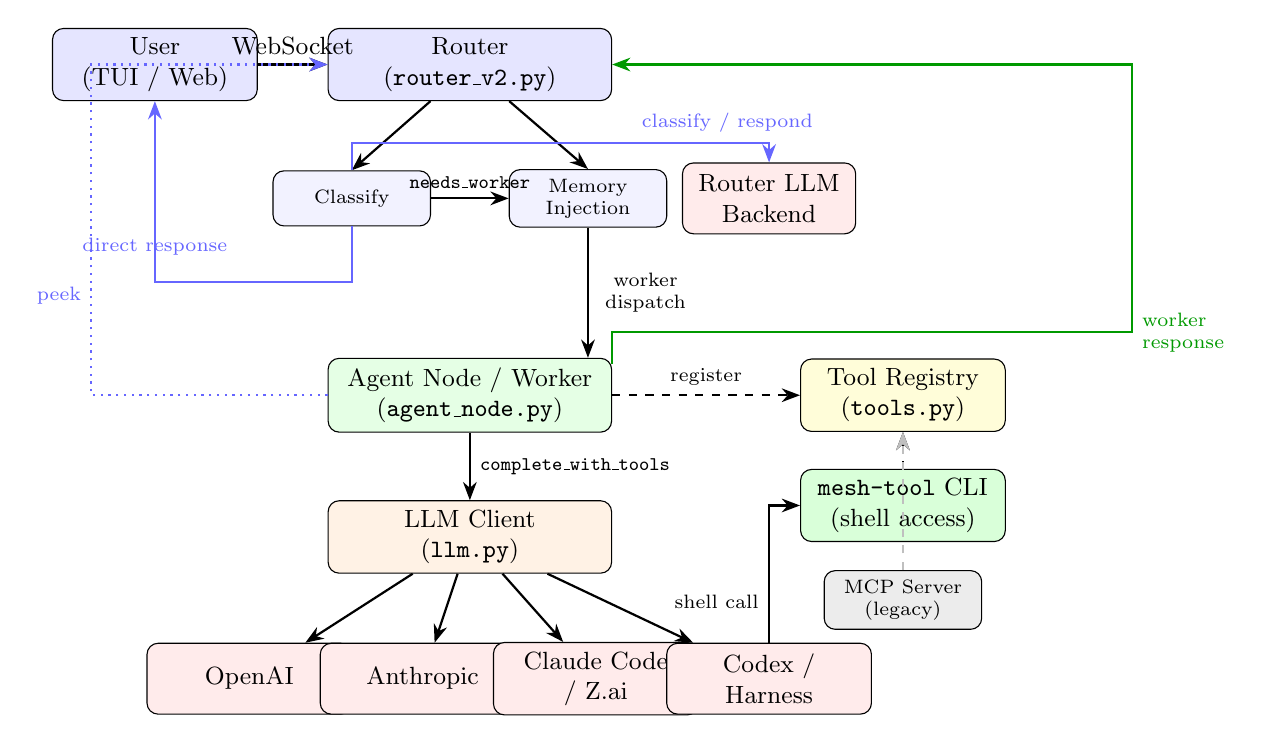
\begin{tikzpicture}[
    >=Stealth,
    box/.style={draw, rounded corners, minimum height=0.9cm,
                minimum width=2.6cm, align=center, font=\small},
    wide/.style={box, minimum width=3.6cm},
    smallbox/.style={draw, rounded corners, minimum height=0.7cm,
                     minimum width=2cm, align=center,
                     font=\scriptsize},
    arrow/.style={->, thick},
    dasharrow/.style={->, thick, dashed},
    every node/.style={font=\small},
  ]

  % Row 0: User + Router
  \node[box, fill=blue!10] at (0, 0) (user) {User\\(TUI / Web)};
  \node[wide, fill=blue!10] at (4, 0) (router)
    {Router\\(\code{router\_v2.py})};

  % Row 1: Router internals + Router's own LLM backend
  \node[smallbox, fill=blue!5] at (2.5, -1.7) (classify)
    {Classify};
  \node[smallbox, fill=blue!5] at (5.5, -1.7) (meminj)
    {Memory\\Injection};
  \node[box, fill=red!8, minimum width=2.2cm] at (7.8, -1.7)
    (routerllm) {Router LLM\\Backend};

  % Row 2: Agent Node
  \node[wide, fill=green!10] at (4, -4.2) (agent)
    {Agent Node / Worker\\(\code{agent\_node.py})};

  % Row 3: Worker LLM Client
  \node[wide, fill=orange!10] at (4, -6) (llm)
    {LLM Client\\(\code{llm.py})};

  % Row 4: Backends
  \node[box, fill=red!8] at (1.2, -7.8) (openai) {OpenAI};
  \node[box, fill=red!8] at (3.4, -7.8) (anthropic) {Anthropic};
  \node[box, fill=red!8] at (5.6, -7.8) (cc) {Claude Code\\/ Z.ai};
  \node[box, fill=red!8] at (7.8, -7.8) (other) {Codex /\\Harness};

  % Tools column (right side, rows 2-4)
  \node[box, fill=yellow!15] at (9.5, -4.2) (tools)
    {Tool Registry\\(\code{tools.py})};
  \node[box, fill=green!15] at (9.5, -5.6) (meshtool)
    {\code{mesh-tool} CLI\\(shell access)};
  \node[smallbox, fill=gray!15] at (9.5, -6.8) (mcp)
    {MCP Server\\(legacy)};

  % Arrows
  \draw[arrow] (user) -- node[above] {WebSocket} (router);
  \draw[arrow] ([xshift=-5mm]router.south) -- (classify.north);
  \draw[arrow] ([xshift=5mm]router.south) -- (meminj.north);
  \draw[arrow] (classify) -- node[above, font=\scriptsize]
    {\code{needs\_worker}} (meminj);
  \draw[arrow, blue!60]
    (classify.north) -- ++(0, 0.35)
    -| node[pos=0.45, above, font=\scriptsize]
    {classify / respond} (routerllm.north);
  \draw[arrow, blue!60]
    (classify.south) -- ++(0, -0.7)
    -| node[pos=0.65, below, font=\scriptsize]
    {direct response} (user.south);
  \draw[arrow, blue!60, dotted]
    (agent.west) -- ++(-3, 0)
    |- node[pos=0.15, left, font=\scriptsize] {peek}
    (router.west);
  \draw[arrow] (meminj.south) --
    node[right, font=\scriptsize, text width=1.2cm, align=center]
    {worker\\dispatch}
    (agent.north -| meminj);
  \draw[arrow] (agent) -- node[right, font=\scriptsize]
    {\code{complete\_with\_tools}} (llm);
  \draw[arrow] (llm) -- (openai);
  \draw[arrow] (llm) -- (anthropic);
  \draw[arrow] (llm) -- (cc);
  \draw[arrow] (llm) -- (other);
  \draw[dasharrow] (agent) -- node[above, font=\scriptsize]
    {register} (tools);
  \draw[arrow] (other.north) |- node[pos=0.15, left,
    font=\scriptsize] {shell call} (meshtool.west);
  \draw[dasharrow] (meshtool) -- (tools);
  \draw[dasharrow, gray!50] (mcp) -- (tools);
  \draw[arrow, green!60!black]
    ([yshift=4mm]agent.east) -- ++(0, 0.4)
    -- ++(6.6, 0)
    node[right, font=\scriptsize, text width=1.3cm, align=left]
      {worker\\response}
    |- (router.east);

\end{tikzpicture}
\caption{Message flow through the mesh.  The router has its own LLM
backend (\code{router\_v2\_llm\_backend}, separate from the worker's)
used for classification and direct response generation (blue arrows).
On \code{needs\_worker}, the router injects relevant memories and
dispatches to the agent node, which calls its own LLM backend via
\code{complete\_with\_tools}.  While a worker is running (BUSY), the
router generates interim responses via worker peek (dotted blue line).
When the worker completes, the agent node sends the response back
through the router to the user (green arrow, right side).
Codex\,/\,Harness subprocesses access mesh tools via the
\code{mesh-tool} CLI.  Dashed lines indicate tool discovery; gray
indicates legacy paths.}
\label{fig:overview}
\end{figure}

Version 2 adds two durable control planes around this message path. The
memory plane turns successful formation batches into internal curation
turns that maintain the digest and entity essays without holding the
message-processing lock. The autonomous plane accepts only runtime-stamped
project wakes, carries a compact \code{SESSION PLAN} across worker-report
continuations, meters dispatch attempts in the router, and commits state to
project dossiers and immutable session reports.

\paragraph{Router states.}
RouterV2 exposes three observable states:
\begin{description}[nosep, leftmargin=1.5em, labelwidth=1.2em]
  \item[IDLE] Incoming message triggers an LLM classification call that
    produces \code{\{needs\_response, needs\_worker\}}.  If
    \code{needs\_worker} is false, the router generates a direct
    response and stays IDLE.  If true, the router sends an immediate
    acknowledgment, injects relevant memories, and spawns a worker.
  \item[BUSY] Worker is running.  New messages are handled by the
    router's own LLM, which peeks at the worker's in-progress
    context to generate contextual interim responses.
  \item[AUTO] An autonomous controller session or one of its scoped worker
    slots is active. The state is derived from trusted session metadata;
    ordinary interactive workers remain BUSY.
\end{description}

\paragraph{Unified harness-backend dispatch.}
When the router's own LLM backend is itself a harness-type backend
(Claude Code, Codex, or \code{mesh-harness}, enumerated in
\code{HARNESS\_BACKENDS} in \code{router\_v2.py}), the router cannot
use native tool calls to launch workers. Instead, these backends share a
unified dispatch contract: router-only tools (\code{worker\_launch},
\code{worker\_status}) are stripped from the effective tool catalog, the
router receives exactly one outer iteration, and the LLM must emit a
\code{<dispatch\_worker>} XML block in its text response to trigger
worker creation. Non-harness backends (e.g., DeepSeek direct API)
retain the native tool-call dispatch path unchanged.

%----------------------------------------------------------------------
\chapter{LLM Backend Dispatch}
\label{ch:backends}
%----------------------------------------------------------------------

Backends are configured in \code{mesh.yaml} under \code{llm\_backends:}
and assigned to agents via the \code{llm\_backend} field on each node.
The \code{LLMClient} class in \code{mesh/llm.py} dispatches to a
backend-specific completion method based on \code{LLMConfig.backend}.

\section{Backend Types}

\begin{table}[h]
\centering
\small
\begin{tabular}{@{}llL{6.5cm}@{}}
\toprule
\textbf{Type} & \textbf{Method} & \textbf{Notes} \\
\midrule
\code{openai}
  & \code{\_complete\_openai} /
    \code{\_complete\_openai\_responses}
  & Two paths: Chat Completions API for standard models;
    Responses API for reasoning models (detected via
    \code{should\_use\_responses\_api}). Supports native
    function calling. \\
\addlinespace
\code{anthropic}
  & \code{\_complete\_anthropic}
  & Claude API with native \code{tool\_use} blocks. Supports
    vision (image extraction from history). \\
\addlinespace
\code{claude-code}
  & \code{\_complete\_claude\_code}
  & Claude Code CLI subprocess. Supports MCP sidecar for
    mesh tools. Multi-account fallback via
    \code{cc\_fallback\_homes}. \\
\addlinespace
\code{zai}
  & \code{\_complete\_zai}
  & Z.ai proxy. Same interface as \code{claude-code}
    (MCP sidecar, CC CLI subprocess). \\
\addlinespace
\code{codex}
  & \code{\_complete\_codex}
  & Codex CLI subprocess with its own built-in tool loop
    (\code{codex:shell}, \code{codex:patch}, etc.).
    Mesh tools available via \code{mesh-tool} CLI on
    \code{PATH} (repo root prepended to subprocess env). \\
\addlinespace
\code{mesh-harness}
  & \code{\_complete\_mesh\_harness}
  & Standalone TAOR (think-act-observe-reflect) loop
    as a subprocess. Usable as any agent backend, not
    only for plan-and-execute. Tool set is configurable
    via \code{harness\_toolset} (see
    Chapter~\ref{ch:harness}). \\
\bottomrule
\end{tabular}
\caption{LLM backend types and their dispatch methods.}
\label{tab:backends}
\end{table}

\section{Live Backend Examples}

The production \code{mesh.yaml} defines 46 backend configurations.
Representative examples:

\begin{table}[h]
\centering
\small
\begin{tabular}{@{}llll@{}}
\toprule
\textbf{Name} & \textbf{Type} & \textbf{Model} & \textbf{Use Case} \\
\midrule
\code{default}              & openai     & gpt-5.1              & General agents \\
\code{openai-reasoning-*}   & openai     & o4-mini / o3         & Reasoning tasks \\
\code{claude-code-opus}     & claude-code & opus                & Most agents \\
\code{deepseek-direct}      & openai     & deepseek-v4-pro      & Memory formation \\
\code{local-qwen36}         & openai     & local-27b            & Local executor (Qwen3.6-27B) \\
\code{codex-5.5}            & codex      & gpt-5.5              & Codex agents \\
\code{mesh-harness-qwen36-pe} & mesh-harness & Qwen3.6-27B + DS-pro & Plan-and-execute \\
\bottomrule
\end{tabular}
\caption{Selected backend configurations from production \code{mesh.yaml}.}
\end{table}

\section{Configuration Reference}
\label{sec:config}

\subsection{Backend Configuration (\code{mesh.yaml})}

Each backend is defined under \code{llm\_backends:} with at minimum:
\begin{lstlisting}
llm_backends:
  my-backend:
    backend_type: openai        # openai | anthropic | claude-code
                                # | zai | codex | mesh-harness
    api_key: ${ENV_VAR}
    base_url: https://...       # optional override
    default_model: gpt-5.1
    max_tokens: 16384
    temperature: 0.7
\end{lstlisting}

\subsection{Agent Node Configuration}

Each agent node under \code{nodes:} references a backend and specifies
tool access:
\begin{lstlisting}
nodes:
  agent:sysadmin:bob:
    nickname: bob
    llm_backend: claude-code-opus
    system_prompt_file: sysadmin.md
    tools: *common_tools           # YAML anchor
    memory_enabled: true
    memory_llm_backend: deepseek-direct
    memory_formation_v3_enabled: true
    memory_retrieval_redesign_enabled: true
\end{lstlisting}

\subsection{Specialized LLM Clients}

Agents may use multiple LLM backends simultaneously:
\begin{itemize}[nosep]
  \item \textbf{Worker backend} (\code{llm\_backend}) ---
        primary LLM for conversation and tool use.
  \item \textbf{Router V2 backend} (\code{router\_v2\_llm\_backend}) ---
        separate LLM for the routing/classification layer.
  \item \textbf{Memory formation backend}
        (\code{memory\_llm\_backend}) --- dedicated LLM for the v3
        segmenter, decoupled from the worker backend (e.g.,
        \code{deepseek-direct} while the worker uses
        \code{claude-code-opus}).
  \item \textbf{Assessor backend} (in plan-and-execute) ---
        the controller/checkpoint LLM, configured per
        \code{mesh-harness} backend definition.
\end{itemize}


%----------------------------------------------------------------------
\chapter{Tool System}
\label{ch:tools}
%----------------------------------------------------------------------

\section{Tool Routing: \code{complete\_with\_tools}}
\label{sec:tool-routing}

The central dispatch method is \code{LLMClient.complete\_with\_tools()}
in \code{mesh/llm.py}. It accepts a \code{ToolRegistry}, a list of
enabled tool names, and optional MCP configuration, then routes based on
backend type.

\subsection{Dispatch Paths}

\begin{figure}[h]
\centering
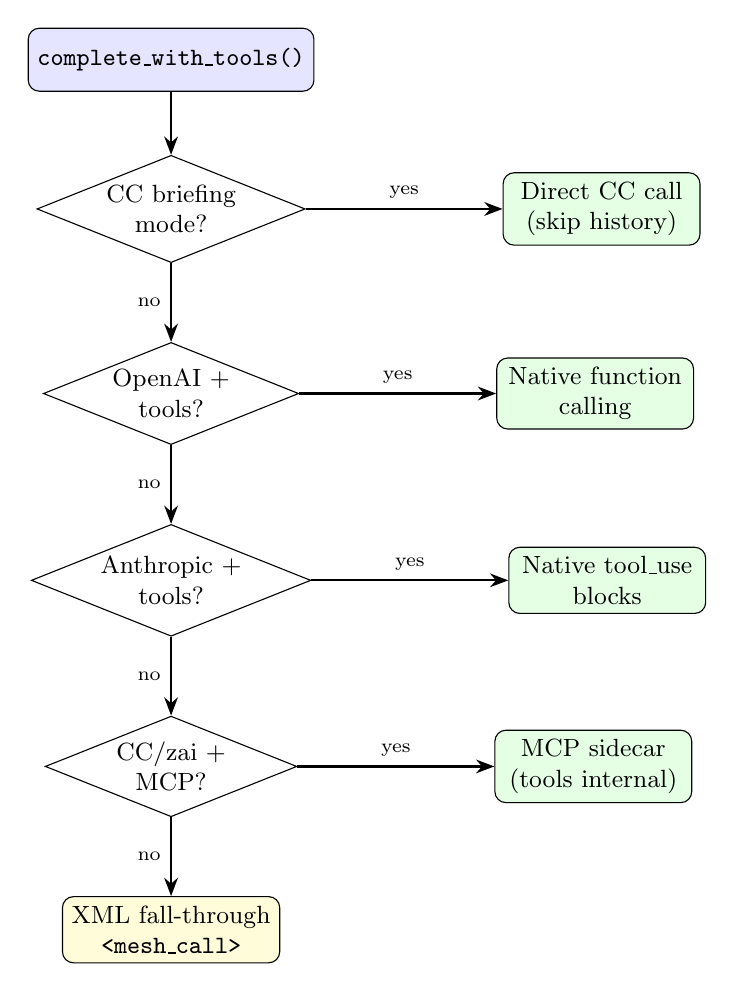
\begin{tikzpicture}[
    >=Stealth,
    decision/.style={diamond, draw, aspect=2.5, inner sep=1pt,
                     font=\small, align=center},
    block/.style={draw, rounded corners, minimum height=0.8cm,
                  minimum width=2.5cm, font=\small, align=center},
    arrow/.style={->, thick},
  ]

  \node[block, fill=blue!10] (entry) {\code{complete\_with\_tools()}};

  \node[decision, below=0.8cm of entry] (d1)
    {CC briefing\\mode?};

  \node[block, fill=green!10, right=2.5cm of d1] (brief)
    {Direct CC call\\(skip history)};

  \node[decision, below=1cm of d1] (d2)
    {OpenAI +\\tools?};

  \node[block, fill=green!10, right=2.5cm of d2] (oai)
    {Native function\\calling};

  \node[decision, below=1cm of d2] (d3)
    {Anthropic +\\tools?};

  \node[block, fill=green!10, right=2.5cm of d3] (ant)
    {Native tool\_use\\blocks};

  \node[decision, below=1cm of d3] (d4)
    {CC/zai +\\MCP?};

  \node[block, fill=green!10, right=2.5cm of d4] (mcp)
    {MCP sidecar\\(tools internal)};

  \node[block, fill=yellow!15, below=1cm of d4] (xml)
    {XML fall-through\\\code{<mesh\_call>}};

  \draw[arrow] (entry) -- (d1);
  \draw[arrow] (d1) -- node[above, font=\scriptsize] {yes} (brief);
  \draw[arrow] (d1) -- node[left, font=\scriptsize] {no} (d2);
  \draw[arrow] (d2) -- node[above, font=\scriptsize] {yes} (oai);
  \draw[arrow] (d2) -- node[left, font=\scriptsize] {no} (d3);
  \draw[arrow] (d3) -- node[above, font=\scriptsize] {yes} (ant);
  \draw[arrow] (d3) -- node[left, font=\scriptsize] {no} (d4);
  \draw[arrow] (d4) -- node[above, font=\scriptsize] {yes} (mcp);
  \draw[arrow] (d4) -- node[left, font=\scriptsize] {no} (xml);

\end{tikzpicture}
\caption{Decision tree in \code{complete\_with\_tools}. The first
matching branch is taken; unmatched backends fall through to XML.}
\label{fig:dispatch}
\end{figure}

\begin{table}[h]
\centering
\small
\begin{tabular}{@{}lL{3cm}L{3.5cm}L{3.5cm}@{}}
\toprule
\textbf{Path} & \textbf{Condition} & \textbf{Tool Format} & \textbf{Response Parsing} \\
\midrule
CC briefing
  & \code{cc\_system\_prompt} \& \code{cc\_user\_prompt} set,
    backend $\in$ \{cc, zai\}
  & None (worker dispatch)
  & Plain text, no tool calls \\
\addlinespace
OpenAI native
  & \code{backend == "openai"} \& tools
  & \code{get\_openai\_tools()} or \code{get\_openai\_responses\_tools()}
  & \code{\_convert\_openai\_tool\_calls()} \\
\addlinespace
Anthropic native
  & \code{backend == "anthropic"} \& tools
  & \code{get\_anthropic\_tools()}
  & \code{\_convert\_openai\_tool\_calls()} \\
\addlinespace
CC/zai + MCP
  & backend $\in$ \{cc, zai\} \& \code{mcp\_config}
    \textbf{[Legacy]}
  & MCP sidecar (tools internal to CC)
  & Plain text; CC executes tools internally.
    Being replaced by \code{mesh-tool} CLI. \\
\addlinespace
XML fall-through
  & Codex, harness, CC/zai without MCP
    \textbf{[Legacy]}
  & \code{format\_tools\_prompt()} $\to$ XML \code{<mesh\_call>} in prompt
  & \code{parse\_tool\_calls()} regex on response.
    Emits \code{DeprecationWarning}. \\
\bottomrule
\end{tabular}
\caption{Tool routing paths in \code{complete\_with\_tools}.}
\label{tab:dispatch}
\end{table}

\subsection{Tool Format Conversion}

The \code{ToolRegistry} (in \code{mesh/tools.py}) provides format
converters for each backend:

\begin{itemize}[nosep]
  \item \code{get\_openai\_tools()} --- OpenAI Chat Completions
        function calling format.
  \item \code{get\_openai\_responses\_tools()} --- OpenAI Responses API
        flattened tool format.
  \item \code{get\_anthropic\_tools()} --- Anthropic \code{tool\_use}
        format.
  \item \code{format\_tools\_prompt()} --- XML
        \code{<mesh\_call>} prompt block for completion-only backends.
\end{itemize}

\section{\code{mesh-tool} CLI}
\label{sec:mesh-tool}

The \code{mesh-tool} CLI provides shell-based access to mesh tools,
replacing the MCP sidecar for all backends with shell access. Any agent
that can execute shell commands can call mesh tools directly, with no schema
injection, XML parsing, or MCP plumbing required.

\paragraph{Architecture.}
\code{mesh-tool} is a bash wrapper at the repository root that activates
the virtualenv and runs \code{python -m mesh.cli.mesh\_tool}. It imports
the same \code{tool\_implementations.py} functions used by the
\code{ToolRegistry} (no reimplementation).

\begin{lstlisting}
mesh-tool (bash wrapper, repo root)
  -> python -m mesh.cli.mesh_tool
     -> imports mesh.tool_implementations
     -> looks up tool in ToolRegistry
     -> parses --key value args (type coercion)
     -> executes handler (async-aware)
     -> JSON to stdout, errors to stderr
\end{lstlisting}

\paragraph{Invocation contract.}
\begin{itemize}[nosep]
  \item \code{mesh-tool} (no args) --- lists all available tools grouped
        by category.
  \item \code{mesh-tool <name>} (no required args provided) --- prints
        usage with required/optional parameters.
  \item \code{mesh-tool <name> -{}-help} --- same as above.
  \item \code{mesh-tool <name> -{}-arg value ...} --- executes the tool.
  \item Wrong/missing arguments --- prints error to stderr with
        ``Did you mean?'' suggestions, usage to stdout, exit~1.
\end{itemize}

\paragraph{Output contract.}
\begin{itemize}[nosep]
  \item \textbf{Success}: JSON to stdout, exit~0.
  \item \textbf{Error}: human-readable message to stderr, usage to
        stdout, exit~1.
  \item \textbf{Help}: usage text to stdout, exit~0.
\end{itemize}

\paragraph{Identity.}
The environment variable \code{MESH\_NODE\_ID} identifies the calling
agent (e.g., \code{agent:sysadmin:bob}). It is propagated through two
layers: (1)~\code{os.environ} is set at agent construction for tool
subprocess inheritance (\code{bash\_exec}, etc.); (2)~\code{LLMConfig.node\_id}
is threaded explicitly into each LLM subprocess environment
(\code{\_run\_cc\_subprocess}, \code{\_complete\_codex},
\code{\_complete\_mesh\_harness}). The explicit path ensures correctness
if multiple agents share a process.

\paragraph{PATH wiring.}
The agent runtime prepends the repository root to \code{PATH} in both
\code{\_run\_cc\_subprocess()} and \code{\_complete\_codex()}, making
\code{mesh-tool} discoverable by any subprocess spawned by these
backends.

\paragraph{Prompt injection.}
All agent prompts auto-include \code{mesh/prompts/mesh\_tools.md} via
the \code{load\_prompt\_file()} auto-include mechanism (same pattern as
\code{channel\_policy.md} and \code{memory.md}). This gives agents
concise instructions on discovering and calling mesh-tool from the shell.

\paragraph{Tool surface.}
53 tools across Gmail, web search, notes, literature,
calendar, memory, maps, mesh info, finance, and utility categories.
Plus \code{send\_message} for agent communication.

\paragraph{Agent-routed tools.}
Tools requiring agent-local state (\code{send\_message},
\code{channel\_list}, \code{mesh\_status}, \code{agent\_status},
\code{schedule\_wake}, \code{gmail\_send\_message},
\code{gmail\_reply\_to}, \code{account\_set\_current},
etc.) are dispatched via the agent's Unix socket
at \code{\textasciitilde/.mesh/sockets/\{sanitized\_id\}.sock}
(directory mode~0700, owner-only access). The CLI falls back to the
legacy \code{/tmp/mesh\_agent\_*} path for agents started before the
hardening change. Memory tools also prefer the socket path when
available.

\paragraph{Gmail account switching.}
All Gmail tools accept an \code{-{}-account} flag for stateless
per-call account selection (e.g., \code{mesh-tool gmail\_list\_recent
-{}-account personal -{}-limit 5}). Each CLI invocation is a fresh
subprocess; there is no persistent account state between calls. Write
tools (\code{gmail\_send\_message}, \code{gmail\_reply\_to}) are routed
through the agent socket with \code{skip\_confirmation=True}; the socket
handler saves the current account, switches to the requested account
before executing, and restores in a \code{try/finally} block.

\paragraph{Stdin mode (shell interpolation hardening).}
When a parameter value is passed as \code{-} and stdin is not a TTY,
\code{mesh-tool} reads the value from standard input instead of from the
command-line argument. This enables single-quoted heredocs to bypass bash
expansion of \code{\$}, backticks, and \code{\$(...)} constructs:

\begin{lstlisting}[numbers=none]
mesh-tool gmail_send_message --to "x@y.com" --subject "Invoice" --body - <<'EOF'
The payment of $550 is still outstanding.
EOF
\end{lstlisting}

Without this mechanism, \code{\$550} would be interpolated as the shell
variable \code{\$5} concatenated with \code{50}, producing a mangled
message. The fix is a three-layer approach: (1) stdin mode in the CLI
parser (\code{mesh\_tool.py}), (2) shell-safety instruction sections in
agent prompts documenting the \code{<<'EOF'} convention, and (3) the
documented convention in \code{mesh/prompts/mesh\_tools.md}.

\paragraph{Map tool socket routing.}
The tools \code{map\_edit}, \code{map\_create}, \code{map\_review}, and
\code{set\_project\_context} are routed through the agent socket via a
prefix-matching check in \code{\_execute()} (not via
\code{AGENT\_ROUTED\_TOOLS}, which is reserved for placeholder-handler
tools). This ensures that worker subprocesses can modify the optional
legacy project-map subsystem via the parent agent's initialized memory system
rather than attempting to initialize their own (which would fail with
``memory not initialized'' errors).

\paragraph{\code{gmail\_list\_recent} / \code{gmail\_list\_unread}.}
Two convenience tools for inbox browsing:
\code{gmail\_list\_recent} returns the $N$ most recent emails (newest
first, no query required), and \code{gmail\_list\_unread} returns
unread emails only. Both accept the \code{-{}-account} flag and are
primarily used by assistant agents for unknown-target email retrieval.

\section{MCP Bridge (Legacy)}
\label{sec:mcp}

\textbf{Status: Being replaced by \code{mesh-tool} CLI
(\S\ref{sec:mesh-tool}).} The MCP sidecar is still functional but is no
longer the recommended path. New agents should use \code{mesh-tool} via
shell instead.

For \code{claude-code} and \code{zai} backends, mesh tools were
historically exposed via an MCP (Model Context Protocol) server sidecar
defined in \code{mesh/mcp\_server.py}. The CC subprocess is started with
\code{-{}-mcp-config} pointing to a temporary JSON file that configures
the MCP server.

\paragraph{Agent-local tools.}
A subset of tools require agent-local state (WebSocket connection,
scheduler, etc.) and are routed to \code{agent\_node.py} via Unix
socket:

\begin{quote}
\small
\code{send\_message}, \code{channel\_list}, \code{channel\_members},
\code{schedule\_wake}, \code{schedule\_list}, \code{schedule\_cancel},
\code{agent\_shutdown}, \code{mesh\_status}, \code{agent\_status}
\end{quote}

\section{Tool Surface}
\label{sec:tools}

\subsection{Mesh Tools}

Mesh tools are defined in \code{mesh/tool\_implementations.py} and
registered via \code{mesh/clients/account\_manager.py} (the
\code{ToolHost}). They cover external services:

\begin{table}[h]
\centering
\small
\begin{tabular}{@{}lL{8cm}@{}}
\toprule
\textbf{Category} & \textbf{Tools} \\
\midrule
Email      & \code{gmail\_list\_from\_date}, \code{gmail\_get\_email},
             \code{gmail\_send\_message}\textsuperscript{S},
             \code{gmail\_reply\_to}\textsuperscript{S},
             \code{gmail\_search\_emails},
             \code{gmail\_list\_recent},
             \code{gmail\_list\_unread} \\
Calendar   & \code{calendar\_list\_on\_date},
             \code{calendar\_create\_event}\textsuperscript{C},
             \code{calendar\_delete\_event}\textsuperscript{C} \\
Notes      & \code{notes\_search}, \code{notes\_list}, \code{notes\_get},
             \code{notes\_read}, \code{notes\_add}, \code{notes\_delete},
             \code{notes\_edit} \\
Web        & \code{exa\_search}, \code{exa\_fetch\_full},
             \code{extract\_url} \\
Literature & \code{literature\_search}, \code{literature\_fulltext},
             \code{arxiv\_\{search,get,fulltext\}},
             \code{pubmed\_\{search,get,fulltext,related\}} \\
Memory     & \code{memory\_\{search,get,list,add,delete\}},
             \code{map\_\{get,list,edit,create,review\}},
             \code{set\_project\_context},
             \code{remember} \\
Finance    & \code{plaid\_\{link\_start,link\_status,accounts,sync,
             transactions,unlink\}} \\
Mesh       & \code{send\_message}, \code{mesh\_list}, \code{mesh\_status},
             \code{agent\_status}, \code{agent\_shutdown},
             \code{channel\_\{list,members\}} \\
Scheduling & \code{schedule\_\{wake,list,cancel\}} \\
Browser    & \code{browser\_\{session\_*,goto,get\_url,snapshot\_controls,
             read\_text,click,fill,type,press,select,back\}} \\
Utility    & \code{current\_time}, \code{tool\_help}, \code{echo},
             \code{account\_\{get\_current,list,set\_current\}},
             \code{personality\_\{get,set\}},
             \code{synthetic\_quota}, \code{claude\_code\_usage} \\
\bottomrule
\end{tabular}
\caption{Mesh tools by category.
  \textsuperscript{S}~=~socket-routed (via agent Unix socket with
  \code{skip\_confirmation}).
  \textsuperscript{C}~=~confirmation-gated (requires user approval).}
\label{tab:mesh-tools}
\end{table}

\subsection{Harness Tools}
\label{sec:harness-tools}

The harness layer (\code{mesh/harness/tools/\_\_init\_\_.py}) defines
three tool sets that mirror or extend the Codex tool surface:

\begin{table}[h]
\centering
\small
\begin{tabular}{@{}lL{4cm}L{5.5cm}@{}}
\toprule
\textbf{Set} & \textbf{Tools} & \textbf{Purpose} \\
\midrule
\code{HARNESS\_TOOLS} (8)
  & \code{apply\_patch}, \code{shell}, \code{list\_dir},
    \code{file\_read}, \code{file\_edit},
    \code{phase\_complete}, \code{grep}, \code{find\_files}
  & Full executor surface. Registered with the global
    \code{ToolRegistry} on import. \\
\addlinespace
\code{PLANNER\_TOOLS} (4)
  & \code{file\_read}, \code{list\_dir}, \code{grep},
    \code{find\_files}
  & Read-only subset for the observe phase. \\
\addlinespace
\code{MESH\_READ\_ONLY\_TOOLS} (45)
  & All read-only mesh tools (search, list, get variants;
    no write/confirmation tools)
  & Safe-to-call during observe phase. Filtered from
    agent's full tool list. \\
\bottomrule
\end{tabular}
\caption{Harness tool sets.}
\label{tab:harness-tools}
\end{table}

\section{Backend--Tool Compatibility Matrix}
\label{sec:matrix}

\begin{table}[h]
\centering
\small
\begin{tabular}{@{}lcccccc@{}}
\toprule
\textbf{Backend} & \textbf{Native} & \textbf{XML}
  & \textbf{MCP} & \textbf{mesh-tool} & \textbf{Mesh Tools}
  & \textbf{Harness} \\
\midrule
\code{openai}       & \checkmark &            &            &             & \checkmark & via harness \\
\code{anthropic}    & \checkmark &            &            &             & \checkmark & via harness \\
\code{claude-code}  &            &            & \dag       & \checkmark  & \checkmark & via harness \\
\code{zai}          &            &            & \dag       & \checkmark  & \checkmark & via harness \\
\code{codex}        &            &            &            & \checkmark  & \checkmark & built-in \\
\code{mesh-harness} &            & \dag       &            & \checkmark  & \checkmark & \checkmark \\
\bottomrule
\end{tabular}
\caption{Backend--tool compatibility. ``Native'' = API-level function
calling. ``XML'' = \code{<mesh\_call>} in prompt. ``MCP'' = tools via
MCP sidecar. ``mesh-tool'' = tools via shell CLI. \dag~=~deprecated
path (still functional but being phased out). ``via harness'' =
available when the backend runs inside the harness layer.
\textbf{Key change}: codex now has mesh tool access via
\code{mesh-tool} CLI.}
\label{tab:matrix}
\end{table}


%======================================================================
%======================================================================
\part{Execution and Control}
\label{part:execution}
%======================================================================
%======================================================================

%----------------------------------------------------------------------
\chapter{The Mesh Harness}
\label{ch:harness}
%----------------------------------------------------------------------

The mesh harness is a standalone TAOR (Think-Act-Observe-Repeat)
execution loop implemented in \code{mesh/harness/loop.py}. It can
operate as a simple iterative executor (standard mode) or as the
substrate for the plan-and-execute controller
(Chapter~\ref{ch:controller}).

\section{Overview}

All harness logic resides in a single file:
\code{mesh/harness/loop.py}. Supporting definitions are in
\code{mesh/harness/tools/\_\_init\_\_.py} (tool sets),
\code{mesh/harness/protocol.py} (event emission), and
\code{mesh/config.py} (configuration plumbing).

The entry point is \code{run\_loop()}, which accepts an LLM client,
conversation history, tool names, and configuration parameters. In
standard mode, it runs a simple loop: call the LLM, execute any tool
calls, append results to history, repeat until the LLM produces a
final response or hits the iteration limit.

\section{Harness Toolset Configuration}
\label{sec:harness-toolset}

The \code{mesh-harness} backend controls which tools the subprocess
receives via two config fields on \code{LLMConfig}:

\begin{itemize}[nosep]
  \item \code{harness\_toolset} (default: \code{"legacy"}) ---
        \code{"legacy"} exposes the full mesh tool set (email, calendar,
        notes, memory, browser, etc.\ via the parent agent's
        \code{ToolRegistry}); \code{"harness"} restricts to the 4-tool
        Codex-style surface (\code{file\_read}, \code{list\_dir},
        \code{grep}, \code{find\_files} plus \code{apply\_patch},
        \code{shell}).
  \item \code{harness\_tools} (default: \code{""}) --- comma-separated
        tool names. When non-empty, \emph{overrides}
        \code{harness\_toolset} entirely, giving fine-grained control.
\end{itemize}

\noindent
The toolset flag is passed to the subprocess via \code{-{}-toolset} or
\code{-{}-tools} CLI arguments (see \code{\_complete\_mesh\_harness()}
in \code{llm.py}).

\paragraph{Codex as direct backend vs.\ through harness.}
There is an important distinction between two ways an agent can use
Codex:
\begin{enumerate}[nosep]
  \item \textbf{Direct backend} (\code{backend\_type: codex}) ---
        \code{\_complete\_codex} launches the Codex CLI subprocess with
        its own built-in tools (\code{codex:shell}, \code{codex:patch},
        etc.).  Mesh tools are now available via \code{mesh-tool} CLI
        on \code{PATH} (repo root prepended to subprocess environment).
  \item \textbf{Through harness} (\code{backend\_type: mesh-harness}
        with a codex sub-backend) --- the harness wraps the Codex model
        in its own TAOR loop and can expose mesh tools via
        \code{harness\_toolset: legacy}.  In this mode, mesh tools are
        available to the harness loop but the inner model does not see
        them directly.
\end{enumerate}

\section{Tool Sets}
\label{sec:tool-sets}

Defined in \code{mesh/harness/tools/\_\_init\_\_.py}:

\begin{table}[h]
\centering
\begin{tabular}{@{}lp{9cm}@{}}
\toprule
Set & Tools \\
\midrule
\code{HARNESS\_TOOLS} &
  \code{apply\_patch}, \code{shell}, \code{list\_dir},
  \code{file\_read}, \code{file\_edit}, \code{phase\_complete},
  \code{grep}, \code{find\_files} \\
\code{PLANNER\_TOOLS} &
  \code{file\_read}, \code{list\_dir}, \code{grep},
  \code{find\_files} \\
\code{MESH\_READ\_ONLY\_TOOLS} &
  45 tools: \code{gmail\_*}, \code{exa\_*}, \code{notes\_*},
  \code{arxiv\_*}, \code{pubmed\_*}, \code{calendar\_*},
  \code{memory\_*}, \code{map\_*}, \code{browser\_*},
  \code{plaid\_*}, etc. \\
\code{READ\_ONLY\_TOOLS} &
  \code{file\_read}, \code{list\_dir}, \code{grep},
  \code{find\_files} (used by degenerate escalation Level~1) \\
\code{WRITE\_TOOLS} &
  \code{apply\_patch}, \code{file\_edit}, \code{file\_create},
  \code{file\_write} (plus shell write pattern detection) \\
\bottomrule
\end{tabular}
\end{table}

\noindent\textbf{Shell write detection.}
\code{\_is\_write\_call()} classifies \code{shell}
calls as writes if their command matches \code{SHELL\_WRITE\_PATTERNS}:

\begin{lstlisting}[numbers=none]
r"\b(sed\s+-i|tee\s|patch\s|mv\s|rm\s|cp\s|chmod\s|
    chown\s|mkdir\s|touch\s)"
r"|[^|]>(?!&)"    # redirect (not pipe)
r"|>>"             # append
\end{lstlisting}

\section{Budget and Limits}
\label{sec:budget}

\begin{table}[h]
\centering
\begin{tabular}{@{}lr@{}}
\toprule
Constant & Default \\
\midrule
\code{MAX\_ITERATIONS} & 100\textsuperscript{\dag} \\
\code{DEFAULT\_SOFT\_LIMIT} & 500{,}000 tokens \\
\code{KEEP\_RECENT\_RESULTS} & 4 \\
\code{FORCED\_SYNTHESIS\_FRACTION} & 0.97 \\
\code{LLM\_RETRIES} & 4 \\
\code{LLM\_RETRY\_BACKOFF} & $(2, 4, 8, 16)$ seconds \\
\code{TRANSIENT\_HTTP\_CODES} & $\{400, 429, 500, 502, 503, 504\}$ \\
\code{CHECKPOINT\_STALL\_TURNS} & 3 \\
\code{DEGENERATE\_ESCALATION\_LIMIT} & 3 \\
\code{DEFAULT\_MAX\_PHASES} & 15 \\
\code{DEFAULT\_COMPACTION\_THRESHOLD\_FRACTION} & 0.40 \\
\code{ASSESSMENT\_MAX\_RETRIES} & 2 \\
\code{PLAN\_MAX\_RETRIES} & 2 \\
\code{HALLUCINATION\_MAX\_RETRIES} & 2 \\
\code{WATCHDOG\_MAX\_CONTEXT\_TOKENS} & 100{,}000 \\
\code{CCWatchdog.RECENT\_WINDOW} & 16 \\
\bottomrule
\end{tabular}
\end{table}

\noindent\textsuperscript{\dag}\code{MAX\_ITERATIONS} is 100 in the code
constant (\code{loop.py:45}), but the CLI \code{-{}-max-iters} flag defaults
to 50 (\code{\_\_main\_\_.py:213}). Agents running without an explicit
\code{-{}-max-iters} argument will hit the 50-iteration limit, not 100.

\subsection{Workspace Calculation}

\begin{align*}
\texttt{workspace} &= \max(\texttt{soft\_limit} - \texttt{initial\_tokens},\ 50{,}000) \\
\texttt{compaction\_threshold} &= \lfloor \texttt{workspace} \times 0.40 \rfloor \\
\texttt{observe\_limit} &= \min(\lfloor \texttt{workspace} \times 0.50 \rfloor,\ 250{,}000)
\end{align*}

\subsection{Effort-to-Budget Mapping}

From \code{mesh/harness/\_\_main\_\_.py}. This maps the \code{cc\_effort}
string to \code{anthropic\_thinking\_budget} (thinking tokens for extended
reasoning), \emph{not} to the context soft limit:

\begin{table}[h]
\centering
\begin{tabular}{@{}lr@{}}
\toprule
Effort & \code{anthropic\_thinking\_budget} (tokens) \\
\midrule
low & 2{,}000 \\
medium & 5{,}000 \\
high & 10{,}000 \\
xhigh & 50{,}000 \\
\bottomrule
\end{tabular}
\end{table}

\noindent The context \code{soft\_limit} is independently configurable via
\code{harness\_soft\_limit} (default: 500{,}000).

\section{Configuration Knobs}
\label{sec:config-knobs}

All P\&E-relevant configuration flows through CLI arguments in
\code{mesh/harness/\_\_main\_\_.py} and the \code{LLMBackendConfig}
class in \code{mesh/config.py}:

\begin{table}[h]
\centering
\begin{tabular}{@{}lll@{}}
\toprule
Config Field & Type & Default \\
\midrule
\code{harness\_controller\_mode} & str & \code{"standard"} \\
\code{harness\_soft\_limit} & int & 500{,}000 \\
\code{harness\_max\_phases} & int & 15 \\
\code{harness\_compaction\_threshold\_fraction} & float & 0.40 \\
\code{harness\_backend} & str & (varies) \\
\code{harness\_toolset} & str & \code{"legacy"} \\
\code{harness\_assessor\_model} & str & (varies) \\
\code{harness\_assessor\_backend} & str & (varies) \\
\code{thinking\_budget}\textsuperscript{*} & int & (none) \\
\code{harness\_assessor\_effort} & str & (none) \\
\code{harness\_codex\_assessor} & bool & false \\
\code{harness\_codex\_assessor\_model} & str & (none) \\
\code{harness\_codex\_assessor\_effort} & str & (none) \\
\code{harness\_codex\_assessor\_binary} & str & \code{"\textasciitilde/.local/bin/codex"} \\
\bottomrule
\end{tabular}
\caption{P\&E configuration fields on \code{LLMBackendConfig}
(\code{mesh/config.py}). \textsuperscript{*}\code{thinking\_budget} lives
on \code{LLMConfig} (\code{mesh/llm.py}), not \code{LLMBackendConfig}; it
is wired through via \code{backend\_config\_to\_llm\_config()}.
In production, \code{harness\_assessor\_effort: xhigh} is set only on
\code{mesh-harness-qwen36-codex-pe}, not on all P\&E backends.}
\end{table}

\noindent\textbf{Checkpoint tuning knobs} (per-call, not config):

\begin{table}[h]
\centering
\begin{tabular}{@{}llr@{}}
\toprule
Parameter & \code{run\_loop()} arg & P\&E default \\
\midrule
Periodic interval & \code{checkpoint\_periodic\_interval} & 5 \\
Periodic start & \code{checkpoint\_periodic\_start} & 8 \\
Stall turns & \code{CHECKPOINT\_STALL\_TURNS} & 3 (hardcoded) \\
Escalation limit & \code{DEGENERATE\_ESCALATION\_LIMIT} & 3 (hardcoded) \\
\bottomrule
\end{tabular}
\end{table}


%----------------------------------------------------------------------
\chapter{Plan-and-Execute Controller}
\label{ch:controller}
%----------------------------------------------------------------------

The Plan-and-Execute (P\&E) controller is a multi-phase execution
controller that wraps the standard TAOR loop with an outer assessor
controller. At each phase boundary, the assessor chooses one of four
intents---\code{observe}, \code{plan}, \code{execute}, or
\code{terminate}.

The controller exists to decompose complex tasks (code edits, bug fixes,
document production) into sequential phases, each with a focused
objective and bounded context. A separate assessor LLM (typically
DeepSeek-v4-pro) drives phase transitions, while the primary LLM
(the executor) performs the actual work within each phase.

\medskip\noindent\textbf{Entry point.}
The P\&E controller is activated when \code{run\_loop()} is called with
\code{controller\_mode="plan\_and\_execute"}. It immediately
delegates to \code{\_run\_plan\_and\_execute\_loop()},
which runs the outer control loop.


\section{Phase Flow}
\label{sec:phase-flow}

\begin{figure}[h]
\centering
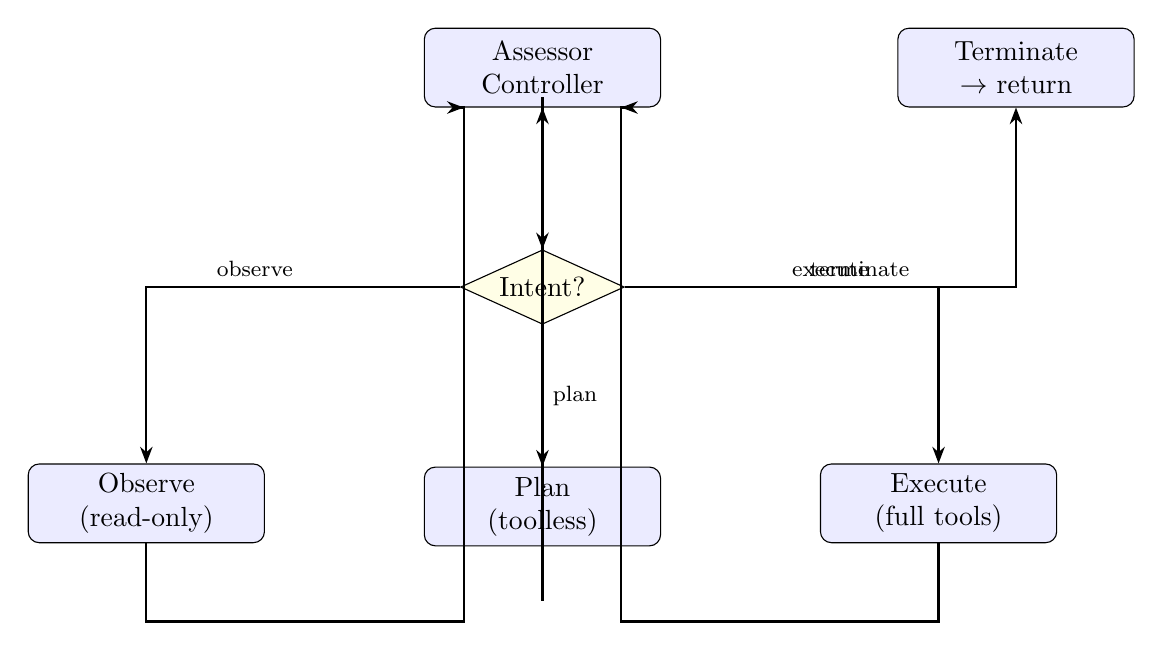
\begin{tikzpicture}[
  node distance=1.8cm and 3cm,
  phase/.style={rectangle, draw, rounded corners, minimum width=3cm,
                minimum height=1cm, align=center, fill=blue!8},
  decision/.style={diamond, draw, aspect=2.2, fill=yellow!10,
                   align=center, inner sep=2pt},
  arrow/.style={-{Stealth[length=6pt]}, thick},
]
  \node[phase] (controller) {Assessor\\Controller};
  \node[decision, below=of controller] (intent) {Intent?};
  \node[phase, below left=2cm and 3cm of intent] (observe) {Observe\\(read-only)};
  \node[phase, below=of intent] (plan) {Plan\\(toolless)};
  \node[phase, below right=2cm and 3cm of intent] (execute) {Execute\\(full tools)};
  \node[phase, right=3cm of controller] (terminate) {Terminate\\$\to$ return};

  \draw[arrow] (controller) -- (intent);
  \draw[arrow] (intent) -| node[above left,pos=0.25]{\footnotesize observe} (observe);
  \draw[arrow] (intent) -- node[right]{\footnotesize plan} (plan);
  \draw[arrow] (intent) -| node[above right,pos=0.25]{\footnotesize execute} (execute);
  \draw[arrow] (intent) -| node[above,pos=0.3]{\footnotesize terminate} (terminate);

  \draw[arrow] (observe) |- ++(0,-1.5) -| ([xshift=-1cm]controller.south) -- (controller);
  \draw[arrow] (plan) -- ++(0,-1.2) -| ([xshift=0cm]controller.south) -- (controller);
  \draw[arrow] (execute) |- ++(0,-1.5) -| ([xshift=1cm]controller.south) -- (controller);
\end{tikzpicture}
\caption{P\&E controller phase flow. Each non-terminal phase loops back
to the assessor controller, which selects the next intent.}
\label{fig:phase-flow}
\end{figure}

The controller iterates up to \code{DEFAULT\_MAX\_PHASES = 15}.
At each iteration, it:

\begin{enumerate}
  \item Builds an evaluator context XML document via
        \code{\_build\_evaluator\_context()}.
  \item Appends an \code{<action\_history>} section summarizing all
        prior phases.
  \item Calls the assessor LLM with the controller template and
        \code{max\_iterations=1} (no tools, single turn).
  \item Parses the response via \code{parse\_controller\_intent()}
        into a \code{ControllerIntent} dataclass.
  \item Dispatches to the appropriate phase handler.
\end{enumerate}

\noindent\textbf{Default on parse failure.}
If the intent tag cannot be parsed, \code{parse\_controller\_intent()}
defaults to \code{observe}---the safest option since it is
read-only.

\noindent\textbf{Phase cap enforcement.}
If the loop exhausts all \code{max\_phases} iterations without
terminating, a hard error message is returned.

\subsection{Phase Tool Exposure}

\begin{table}[h]
\centering
\small
\begin{tabular}{@{}llL{6cm}@{}}
\toprule
\textbf{Phase} & \textbf{LLM} & \textbf{Available Tools} \\
\midrule
Controller (assessor)
  & Assessor (e.g., DS-pro)
  & \code{tool\_names=[]} --- no tools; emits XML intent only \\
\addlinespace
Observe
  & Executor backend
  & \code{PLANNER\_TOOLS} $\cup$
    (agent's \code{tool\_names} $\cap$
    \code{MESH\_READ\_ONLY\_TOOLS}) \\
\addlinespace
Plan
  & Controller LLM
  & \code{tool\_names=[]} --- single call, parses plan XML \\
\addlinespace
Execute
  & Executor backend
  & Full agent \code{tool\_names}
    (all configured tools $+$ \code{HARNESS\_TOOLS}) \\
\bottomrule
\end{tabular}
\caption{Tool exposure per plan-and-execute phase. The observe phase
cannot trigger write or confirmation-gated tools.}
\label{tab:phase-tools}
\end{table}

\begin{figure}[h]
\centering
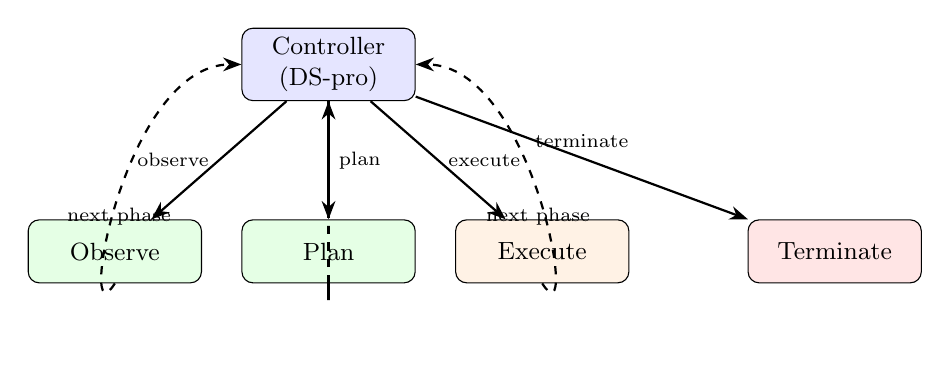
\begin{tikzpicture}[
    >=Stealth,
    box/.style={draw, rounded corners, minimum height=0.8cm,
                minimum width=2.2cm, align=center, font=\small},
    arrow/.style={->, thick},
  ]

  \node[box, fill=blue!10] (ctrl) {Controller\\(DS-pro)};
  \node[box, fill=green!10, below left=1.5cm and 0.5cm of ctrl]
    (obs) {Observe};
  \node[box, fill=green!10, below=1.5cm of ctrl]
    (plan) {Plan};
  \node[box, fill=orange!10, below right=1.5cm and 0.5cm of ctrl]
    (exec) {Execute};
  \node[box, fill=red!10, right=1.5cm of exec]
    (term) {Terminate};

  \draw[arrow] (ctrl) -- node[left, font=\scriptsize] {observe} (obs);
  \draw[arrow] (ctrl) -- node[right, font=\scriptsize] {plan} (plan);
  \draw[arrow] (ctrl) -- node[right, font=\scriptsize] {execute} (exec);
  \draw[arrow] (ctrl) -- node[above, font=\scriptsize] {terminate} (term);

  \draw[arrow, dashed] (obs.south) .. controls +(-0.5,-0.8) and
    +(-1.5,0) .. node[below, font=\scriptsize] {next phase} (ctrl.west);
  \draw[arrow, dashed] (plan.south) .. controls +(0,-0.8) and
    +(0,-1.5) .. node[below, font=\scriptsize] {} (ctrl.south);
  \draw[arrow, dashed] (exec.south) .. controls +(0.5,-0.8) and
    +(1.5,0) .. node[below, font=\scriptsize] {next phase} (ctrl.east);

\end{tikzpicture}
\caption{Controller loop. Each phase feeds back to the controller
for the next intent decision. Terminate exits the loop and returns
the final response.}
\label{fig:controller}
\end{figure}


\section{Assessor Controller}
\label{sec:assessor}

The assessor is a separate LLM client (\code{assessor\_llm\_client}),
defaulting to the primary \code{llm\_client} if not provided.
In production this is typically DeepSeek-v4-pro.

\subsection{Controller Invocation}

The controller is invoked as a \emph{single-turn, toolless}
\code{run\_loop()} call:

\begin{lstlisting}
controller_output = await run_loop(
    llm_client=_assessor,
    history=[HistoryMessage(
        from_node="user",
        content=eval_ctx,     # evaluator context XML
        ...)],
    tool_names=[],            # no tools
    max_iterations=1,         # single turn
    instructions=phase_instructions,  # controller template
    ...
)
\end{lstlisting}

The controller sees a fresh single-message history containing only the
evaluator context; it does not share the executor's conversation history.

\subsection{Controller Template}

The template (\code{\_CONTROLLER\_TEMPLATE}) presents
four intents with XML output format:

\begin{itemize}[nosep]
  \item \code{<intent>observe</intent>} + \code{<prompt>}
  \item \code{<intent>plan</intent>} + \code{<plan>}
  \item \code{<intent>execute</intent>} + \code{<prompt>}
  \item \code{<intent>terminate</intent>} + \code{<summary>}
\end{itemize}

\subsection{Evaluator Context}
\label{sec:eval-context}

The function \code{\_build\_evaluator\_context()}
constructs an XML document:

\begin{lstlisting}[language=XML,numbers=none]
<evaluator_context>
  <task>...</task>
  <plan>...</plan>            <!-- current plan, if any -->
  <prior_phases>              <!-- compacted phase summaries -->
    <phase_summary phase="N">...</phase_summary>
  </prior_phases>
  <current_phase phase="N">
    <objective>...</objective>
    <tool_history>            <!-- faithful tool call/result copies -->
      <tool_call name="...">...</tool_call>
    </tool_history>
    <files_modified>...</files_modified>
  </current_phase>
  <action_history>            <!-- appended by P&E loop -->
    - Phase 1 (observe): ...
    - Phase 2 (plan): ...
  </action_history>
</evaluator_context>
\end{lstlisting}

Prior phase summaries are populated either from an explicit list or by
scanning history messages for \code{<phase\_summary>} tags.
Files modified are tracked by matching
\code{WRITE\_TOOLS} tool names and extracting file paths via regex.


\section{Triage}
\label{sec:triage}

\textbf{Note:} Triage is \emph{not} currently invoked by the P\&E
controller loop. \code{\_TRIAGE\_TEMPLATE} and
\code{parse\_triage()} exist in the codebase but
the P\&E loop does not call them; the first phase simply goes to the
controller for an intent decision. The controller template's guidelines
(``If the task is a simple factual question you can answer now, terminate
immediately'') serve the same purpose implicitly.

Triage classifies tasks into three categories:
\begin{enumerate}[nosep]
  \item \textbf{Done} --- answerable from knowledge, no tools needed.
  \item \textbf{Search-only} (\code{needs\_plan=false}) --- pure
        information retrieval; findings are the deliverable.
  \item \textbf{Needs plan} (\code{needs\_plan=true}) --- requires
        producing an artifact (code, documents, etc.).
\end{enumerate}

The \code{TriageDecision} dataclass captures the
parse result. On parse failure, \code{parse\_triage()} defaults to
\code{needs\_plan=True}.


\section{Observe Phase}
\label{sec:observe}

When the controller selects \code{observe}, the executor runs a
read-only exploration loop:

\begin{itemize}[nosep]
  \item \textbf{Tools:} \code{search\_tools} = \code{PLANNER\_TOOLS}
        (\code{file\_read}, \code{list\_dir}, \code{grep},
        \code{find\_files}) plus any \code{MESH\_READ\_ONLY\_TOOLS}
        found in the task's \code{tool\_names}.
  \item \textbf{Soft limit:}
        $\texttt{observe\_limit} = \min(\lfloor\texttt{workspace} \times 0.50\rfloor, 250{,}000)$.
  \item \textbf{Checkpoints:} enabled, with
        \code{checkpoint\_periodic\_interval=5},
        \code{checkpoint\_periodic\_start=8}.
  \item \textbf{Instructions:} \code{OBSERVE\_INSTRUCTIONS}
        appended to the controller's prompt.
\end{itemize}

\noindent\textbf{No compaction after observe.}
History from observe phases is preserved intact so that subsequent
plan/execute phases can see the raw tool results
(commit \code{d8d74ca5}).

\noindent\textbf{Phase discipline is advisory, not enforced.}
The observe phase uses \code{PLANNER\_TOOLS} (read-only) but this is
enforced only at the tool-set level. If the executor's backend (e.g.,
Claude Code) has its own tools, those are not restricted by the harness
tool-name filter.


\section{Plan Phase}
\label{sec:plan}

When the controller selects \code{plan}, the plan is extracted
inline from the controller's own output; no separate LLM call is made.
The plan is stored in \code{current\_plan} and injected into subsequent
executor phases via \code{\_EXECUTOR\_FRAMING} and
into assessments via \code{\_ASSESSMENT\_TEMPLATE}.

\noindent\textbf{Plan revision.}
The controller can revise the plan at any time by selecting
\code{plan} again. Additionally, the legacy assessment path supports
\code{<revised\_plan>} tags that replace \code{current\_plan}.

\noindent\textbf{Relationship to legacy plan phase.}
The \code{PLAN\_INSTRUCTIONS} template and
\code{extract\_plan\_and\_phase\_prompt()} are
remnants of the earlier fixed-sequence controller (observe $\to$ plan
$\to$ execute). In the current assessor-controller design, the plan
phase is handled inline by the controller itself, and these functions are
not called by the P\&E loop.


\section{Execute Phase}
\label{sec:execute}

When the controller selects \code{execute}, a full-power TAOR loop
runs:

\begin{itemize}[nosep]
  \item \textbf{Tools:} the original \code{tool\_names} passed to
        \code{run\_loop()} (typically \code{HARNESS\_TOOLS} plus
        mesh read/write tools).
  \item \textbf{Soft limit:} the full \code{soft\_limit} (not the
        reduced observe limit).
  \item \textbf{Instructions:} \code{\_EXECUTOR\_FRAMING} template
        wraps the controller's prompt with plan context.
  \item \textbf{Checkpoints:} enabled, \code{periodic\_interval=5},
        \code{periodic\_start=8}.
  \item \textbf{CCWatchdog:} enabled for \code{claude-code} and
        \code{zai} backends when \code{assessor\_llm\_client} is
        provided.
\end{itemize}

\subsection{Executor Framing}

The executor receives its instructions via \code{\_EXECUTOR\_FRAMING},
which injects the current plan and phase-specific goal into a structured
template. The framing tells the executor to focus only on the current
phase's goal and not to start the next phase.


\section{Observe Cap}
\label{sec:observe-cap}

After 2 observe phases (lifetime, not per-segment), the observe intent
is disabled. This is a two-layer enforcement (commit \code{bb62ff3c}):

\subsection{Layer 1: Template Swap}

When \code{observe\_count >= 2}, the controller template is replaced
with \code{\_CONTROLLER\_TEMPLATE\_NO\_OBSERVE} via
\code{\_strip\_observe\_from\_instructions()}. The
no-observe template begins with:

\begin{quote}
\itshape
\textbf{observe is temporarily disabled} --- you have already used your
observation budget. Choose plan, execute, or terminate.
\end{quote}

If the template swap fails (template not found in instructions), a
\code{RuntimeError} is raised as a drift-protection mechanism.

\subsection{Layer 2: Hard Enforcement}

If the assessor LLM ignores the template and returns \code{observe}
anyway, the phase is \emph{skipped} (not force-terminated). A warning is
logged and the action history records the skip.

\noindent\textbf{Lifetime cap.}
The \code{observe\_count} is incremented on each observe phase
and is \emph{never reset}---not even after execute phases. The cap
is lifetime, not per-segment.

\section{Safety Properties}

\begin{itemize}[nosep]
  \item \textbf{Observe cap}: After 2 observe phases, the observe
        intent is permanently removed from the controller's option set
        for the remainder of the task.
  \item \textbf{Observe checkpoints}: Every 5 iterations starting at
        iteration 8, the assessor is asked whether to continue or
        complete the phase.
  \item \textbf{History carryover}: Observe-phase tool results
        (file reads, searches) are preserved in the shared
        \code{history} list for subsequent phases. No compaction fires
        between observe and execute; only between consecutive execute
        phases.
  \item \textbf{Read-only observe}: The \code{MESH\_READ\_ONLY\_TOOLS}
        whitelist ensures the observe phase cannot send emails, create
        events, or perform other write operations.
\end{itemize}


\section{Key Commits}
\label{sec:commits}

\begin{description}[style=nextline,leftmargin=0pt]
  \item[\code{54a33f8a}]
    \textit{feat: plan-and-execute controller, codex backend, assessor
    streaming, greenfield benchmarks.}
    Initial P\&E implementation with fixed observe $\to$ plan $\to$
    execute sequence and assessor-driven phase transitions.

  \item[\code{c4bc1763}]
    \textit{feat: flexible assessor controller, synthesis/compaction
    dead-zone fix, gpt-oss reasoning fallback.}
    Replaced fixed sequence with flexible four-intent controller
    (observe/plan/execute/terminate).

  \item[\code{bb62ff3c}]
    \textit{fix: P\&E controller --- lifetime observe cap,
    skip-not-force semantics, helpers.}
    Changed observe cap from per-segment to lifetime.

  \item[\code{d8d74ca5}]
    \textit{fix: preserve observe-phase history for executor --- stop
    compacting between phases.}

  \item[\code{177d8689}]
    \textit{feat(harness): per-turn context budget meter + forced-synthesis cutoff.}
    Added continuous budget awareness line and the forced synthesis
    mechanism.
\end{description}


%----------------------------------------------------------------------
\chapter{Native Multi-Turn Executor Loop}
\label{ch:native-loop}
%----------------------------------------------------------------------

The XML-serialized history path (\code{run\_loop}) has a fundamental
deficiency for multi-phase execution: tool results from prior phases appear
to the executor as \code{<message from="system">} XML text rather than
native API tool results. The executor model treats them as someone else's
notes and re-reads the same files, duplicating context and accelerating
compaction.

The native executor loop (\code{run\_native\_loop}) solves this
by maintaining the conversation as a native OpenAI \code{messages:
list[dict]} instead of \code{list[HistoryMessage]}. Tool results are
stored as \code{\{"role": "tool", "tool\_call\_id": "..."\}} messages; the
executor treats them as its own prior work and builds on them across phase
boundaries.

\section{Location}

\begin{description}[style=nextline]
  \item[\code{mesh/harness/loop.py}]
    \code{run\_native\_loop()}, plus helper functions
    \code{estimate\_native\_tokens()},
    \code{\_tool\_name\_for\_call\_id()},
    \code{\_build\_evaluator\_context\_from\_native()},
    \code{\_compact\_native\_history()}.
  \item[\code{mesh/llm.py}]
    \code{complete\_multi\_turn()}---OpenAI Chat
    Completions call that accepts pre-built \code{messages} and skips
    XML serialization entirely.
  \item[\code{mesh/tools.py}]
    \code{ToolCall.call\_id} field, which preserves the API-returned tool call
    ID for native message linking.
\end{description}

\section{Activation}

Native mode activates when \code{backend == "openai"} inside
\code{\_run\_plan\_and\_execute\_loop()}. Non-OpenAI backends
(CC, zai, mesh-harness XML) fall back to the existing XML path. The
dispatch is purely conditional, requiring no configuration flag.

\section{Message Format}

The conversation uses standard OpenAI Chat Completions format:

\begin{lstlisting}
# System + task (protected zone, never compacted)
{"role": "system", "content": "<system_prompt + tool_prompt>"}
{"role": "user",   "content": "<task + instructions>"}

# Phase framing (injected by P&E controller before each phase)
{"role": "user",   "content": "<observe/execute instructions>"}

# Assistant turn with tool calls
{"role": "assistant", "tool_calls": [
    {"id": "call_abc", "type": "function",
     "function": {"name": "file_read", "arguments": "..."}}
]}
# Tool result linked by call_id
{"role": "tool", "tool_call_id": "call_abc",
 "content": "<file contents>"}
\end{lstlisting}

\section{Cross-Phase Carry-Forward}

The \code{native\_messages} list is shared across observe and execute
phases via the P\&E controller. When the assessor transitions from observe
to execute:
\begin{enumerate}
  \item Observe phase tool results remain in \code{native\_messages} as
    native \code{role=tool} messages.
  \item The P\&E controller appends the executor framing as a
    \code{role=user} message.
  \item The execute phase calls \code{run\_native\_loop()} with the same
    \code{native\_messages} list.
  \item The executor LLM sees all observe-phase file reads as its own prior
    tool results and does not re-read them.
\end{enumerate}

\section{Per-Iteration Budget Injection}

On each iteration, \code{run\_native\_loop} appends a transient
\code{role=user} message containing the budget line and any per-iteration
instructions. This message is removed after the LLM responds so it does
not accumulate in the conversation history. During forced synthesis, the
message stays (it is the final instruction to produce output).

\section{Assessor Boundary}

The assessor remains on the XML path. When the P\&E controller needs a
phase decision:
\begin{enumerate}
  \item \code{\_build\_evaluator\_context\_from\_native()} converts the
    native messages into structured XML (\code{<evaluator\_context>}).
  \item The assessor call uses \code{run\_loop} (XML mode) with a
    single-message history containing the evaluator context.
  \item The assessor never sees native messages directly.
\end{enumerate}

This separation is intentional: the assessor needs a structured bird's-eye
view for phase decisions, while the executor needs native tool context for
implementation work.

\section{Compaction in Native Mode}

When scratchpad tokens exceed \code{compaction\_threshold} after an execute
phase:
\begin{enumerate}
  \item \code{\_compact\_native\_history()} is called with
    \code{compact\_after} (protected zone boundary).
  \item A split-safety guard walks backward from \code{compact\_after} to
    ensure it does not bisect an assistant$\to$tool\_result group (would
    create orphaned tool\_calls or dangling tool results).
  \item Compactable messages are serialized to text and sent to the LLM
    via \code{complete\_with\_tools} (XML path) for summarization.
  \item The compactable region is replaced by a single
    \code{<phase\_summary>} user message.
  \item \code{last\_native\_phase\_start\_idx} is set to
    \code{len(native\_messages)} after compaction to avoid stale indices.
\end{enumerate}

\section{\code{complete\_multi\_turn} Method}

Located in \code{mesh/llm.py}, this method:
\begin{itemize}
  \item Accepts \code{messages: list[dict]} in OpenAI format.
  \item Passes them verbatim to the Chat Completions API (no XML
    serialization).
  \item Accepts pre-converted \code{tools: list[dict]} from
    \code{ToolRegistry.get\_openai\_tools()}.
  \item Handles reasoning effort negotiation (xhigh$\to$high fallback,
    non-reasoning model stripping).
  \item Returns \code{(content, tool\_calls, usage)}.
  \item \code{parallel\_tool\_calls} parameter (default \code{True})
    controls whether the API is allowed to issue multiple tool calls per
    turn.
\end{itemize}

\section{Protocol Events}

The native loop emits the same protocol events as the XML loop:
\begin{itemize}
  \item \code{emit\_tool\_call(name, arguments, call\_id)} before each tool
    execution.
  \item \code{emit\_tool\_result(name, result, call\_id, success)} after
    each tool execution.
  \item \code{emit\_turn\_started}, \code{emit\_assistant\_message},
    \code{emit\_thread\_started/finished}, checkpoint events.
\end{itemize}


%----------------------------------------------------------------------
\chapter{Autonomous Project Controller}
\label{ch:autonomous-controller}
%----------------------------------------------------------------------

The v2 autonomous controller is distinct from the harness P\&E controller.
P\&E chooses phases inside one execution task; autonomous agent mode advances
a durable project across bounded sessions. It uses the ordinary router and
worker-dispatch machinery but adds trusted project scope, a project dossier,
immutable session reports, persistent attempt budgets, and deterministic
wake scheduling.

\section{Enrollment and Trusted Session Scope}

Enrollment is explicit in \code{mesh.yaml}. A node enables
\code{autonomous\_agent\_mode\_enabled}, lists the exact
\code{autonomous\_projects} it controls, and sets a per-session worker
ceiling and active-mode pacing gap. The public example configuration shows
the surface without shipping a live deployment.

The controller mandate is not placed unconditionally in every prompt.
\code{AgentNode.autonomous\_wake\_metadata()} recognizes the canonical
\code{[AUTONOMOUS PROJECT SESSION]} header, validates the named
\code{project:*} key against that node's enrollment, caps the requested
session limit to configuration, and mints a session ID. Only this
runtime-stamped metadata activates the planning mandate. A user message that
merely imitates the header cannot enroll a project or mint a trusted session.
Worker-report continuations receive the execute-and-close mandate rather than
restarting the planning phase.

\section{Durable Project Dossier}

\code{mesh/project\_dossier.py} defines the project state authority. Each
dossier is a Markdown document under \code{\textasciitilde/.mesh/digests/}
with frontmatter and exactly seven ordered, non-empty sections:

\begin{enumerate}[nosep]
  \item Identity,
  \item Goals,
  \item Tasks,
  \item Timeline,
  \item Narrative,
  \item Standing decisions, and
  \item Open threads.
\end{enumerate}

Task rows live inside a schema-marked block and carry stable task IDs,
pending/in-progress/done status, priority, goal linkage, and completion
evidence. A validator checks identity, structure, the optional project-model
block, and the global token ceiling before an exact-string edit lands.
Writes use a same-directory temporary file, \code{fsync}, and rename; a
failed validation leaves the prior dossier byte-identical. Initialization is
create-once and never overwrites an existing dossier.

The controller is the sole routine dossier writer. Workers receive the
dossier as read-only project context and return claims plus artifacts; they do
not edit project state, write reports, or schedule more work. This separates
execution evidence from the component that decides task transitions.

\section{One Bounded Session}

The shipped mandates
(\code{mesh/prompts/autonomous\_controller.txt} and
\code{autonomous\_controller\_execute.txt}) define a two-phase protocol:

\begin{enumerate}
  \item \textbf{Plan.} Check the daily ledger, read the dossier, follow only
        relevant report/memory links, repair the task roster, and write a
        bounded \code{SESSION PLAN}. The plan names a goal, ordered task IDs,
        completion evidence, and the first action before any worker launch.
  \item \textbf{Execute and close.} Mark the selected task in progress,
        dispatch a self-contained worker brief, verify the resulting artifacts
        and tests, and continue only while both session and daily headroom
        remain. Direction-changing evidence is recorded in the dossier before
        another dispatch. Closeout writes the immutable report, indexes a
        compact memory pointer, updates live dossier state and the standing
        digest, relays the scheduler decision, and stops.
\end{enumerate}

The router captures a schema-valid \code{SESSION PLAN} (four required fields,
at most ten lines and 4,000 characters) on the outgoing planning turn. It
stamps that bounded copy into trusted session metadata, then carries it on
worker completion even if rolling conversation history has been summarized or
dropped. A continuation without a valid carrier receives an explicit
\code{SESSION PLAN UNAVAILABLE} recovery instruction rather than an invented
plan.

\section{Immutable Reports and Audit Chain}

\code{dossier\_write\_report} creates a dated, sequenced report beneath
\code{\textasciitilde/.mesh/reports/} and links it from the dossier Timeline.
An identical retry is idempotent; different bytes at an existing report path
are refused, so corrections require a later amendment report. The mandate
requires the session plan, worker reports verbatim, controller verification,
decisions, artifacts, issues, budget use, and next-wake intent. The report is
the audit authority; the dossier is the current-state authority; episodic
memory stores only a compact pointer back to the canonical report.

\section{Admission Budgets and Single-Writer Boundaries}

The daily project ledger is a JSON file beneath
\code{\textasciitilde/.mesh/budget/}. Its limit comes from dossier
frontmatter; the dated \code{used} counter rolls over on a new day. The
central dispatch seam in \code{RouterV2} is the sole normal-path charger:

\begin{enumerate}[nosep]
  \item trusted session scope mechanically supplies a
        \code{[PROJECT: project:...]} tag when the model omitted it;
  \item duplicate, capacity, and selection refusals run before the budget
        check and consume nothing;
  \item an admitted dispatch is charged exactly once at reservation, before
        worker startup; and
  \item a failed start is deliberately not refunded, because budgets bound
        attempts and must also bound retry storms.
\end{enumerate}

The controller therefore reads \code{dossier\_check\_budget} but must never
call \code{dossier\_spend\_budget}; doing so would double-charge the same
attempt. Exhaustion returns a structured, final refusal. A ledger-write
failure after admission is logged as an understated count, and a missing tag
or unreadable budget ledger fails open with a warning. Thus ``one charge per
attempt'' is the validated normal path, while infrastructure failure is made
observable rather than falsely represented as enforcement.

The operator can change the configured daily ceiling through the brokered
control surface. The sibling \code{budget-reset} operation clears only the
current day's \code{used} count; it does not change the limit. Dossier files,
immutable reports, ledgers, and scheduled wakes are all stored on disk, so a
process restart reloads rather than reconstructs project state.

\section{Active Mode and Scheduled Wakes}

Active mode is opt-in per project. After a successful report write,
\code{AgentNode} calls the pure decision function in
\code{mesh/autonomous\_active.py}. It schedules no wake unless the dossier's
active flag is true, daily budget remains, the last report is non-terminal,
and no wake for that project is already pending. A minimum gap (60 minutes by
default) paces sessions. If another wake for the same agent would overlap,
the candidate is moved beyond it. The result is one explicit one-shot wake,
not a recurrence; every closeout re-evaluates all gates from fresh state.

Reports with status \code{blocked}, \code{failed}, or \code{no\_op} suppress
automatic continuation. Pending wakes live in the agent's SQLite store and
are reloaded at startup. The controller does not choose or override the
runtime's timestamp: it reports the returned wake ID or the reason that no
wake was scheduled.

\section{Operator Surface}

Autonomous controls use \code{AUTONOMOUS\_CONTROL} messages routed through
the central router and independently revalidated by the enrolled agent. The
TUI exposes:

\begin{table}[h]
\centering
\small
\begin{tabular}{@{}lL{8cm}@{}}
\toprule
\textbf{Command} & \textbf{Effect} \\
\midrule
\code{/auto} & Fan out status for enrolled controllers: projects, budgets,
  active flags, pending wakes, and current session. \\
\code{/auto wake <agent> [<project>] [<time>]} & Schedule a bounded project
  session; omitting time means immediate. \\
\code{/auto budget <project> <n>} & Set the daily worker ceiling (1 to 50). \\
\code{/auto budget <project> reset} & Clear today's spent-attempt count while
  retaining the ceiling. \\
\code{/auto active <project> on|off} & Arm or disarm paced automatic
  continuation. \\
\code{/auto cancel <agent> <wake-id>} & Cancel a pending wake. \\
\code{/wake [project]} & Convenience form that resolves the project's owner
  and starts a session immediately. \\
\code{/report [project] [since YYYY-MM-DD]} & Request a report-oriented
  autonomous writing session. \\
\bottomrule
\end{tabular}
\caption{Autonomous controller operations in \code{run\_user\_tui.py}.}
\label{tab:auto-commands}
\end{table}


%----------------------------------------------------------------------
\chapter{Context Management}
\label{ch:context}
%----------------------------------------------------------------------

\section{Forced Synthesis}
\label{sec:forced-synthesis}

Forced synthesis is a budget-exhaustion mechanism in the \emph{inner}
TAOR loop (\code{run\_loop()}).

\begin{align*}
\texttt{synthesis\_threshold} &= \lfloor \texttt{soft\_limit} \times 0.97 \rfloor
\end{align*}

At each iteration, \code{estimate\_history\_tokens(history)} is
compared against the threshold. When exceeded:

\begin{enumerate}[nosep]
  \item All tools are stripped (\code{effective\_tool\_names = []}).
  \item The instructions are replaced with a forced-synthesis message
        directing the model to produce its final response immediately.
  \item A budget line is prepended showing current and maximum token
        counts.
  \item An error event is emitted (non-fatal).
\end{enumerate}

The budget line is injected on \emph{every} iteration,
even before forced synthesis triggers, giving the model continuous
awareness of context consumption.


\section{Compaction}
\label{sec:compaction}

\subsection{When It Fires}

Compaction runs \emph{only after execute phases}.
It fires when:
\[
\texttt{scratchpad\_tokens} = \texttt{estimated\_tokens} - \texttt{initial\_tokens} > \texttt{compaction\_threshold}
\]
where:
\begin{align*}
\texttt{workspace} &= \max(\texttt{soft\_limit} - \texttt{initial\_tokens},\ 50{,}000) \\
\texttt{compaction\_threshold} &= \lfloor \texttt{workspace} \times 0.40 \rfloor
\end{align*}

\noindent\textbf{No compaction after observe phases.}
This was an intentional fix (commit \code{d8d74ca5}) to preserve raw
observation data for the planner.

\subsection{Protected Zone}

\code{compact\_after} marks the boundary between protected
and compactable history. It is set to the initial history length and
never moves. Everything before \code{compact\_after} (the original
task prompt) is never touched.

\subsection{Compaction Procedure}

The function \code{\_compact\_history()}:

\begin{enumerate}[nosep]
  \item Concatenates all messages after \code{compact\_after} into a
        single string.
  \item Formats \code{\_COMPACTION\_TEMPLATE}
        with the phase prompt and appends the raw text.
  \item Calls the primary LLM (not the assessor) with a fresh
        single-turn conversation.
  \item Extracts content from \code{<phase\_summary>} tags if present.
  \item Deletes all messages after \code{compact\_after} and inserts a
        single summary message.
\end{enumerate}

The compaction template instructs the LLM to preserve five categories:
actions attempted, successes and key facts, failures with verbatim error
messages, artifacts produced, and open sub-questions.

\noindent\textbf{Failure mode.}
If the compaction LLM call fails, the first 2000 characters of
\code{executor\_output} are preserved as a fallback.


\section{Degenerate Loop Detection}
\label{sec:degenerate}

The checkpoint system detects and responds to degenerate executor
behavior (reading the same files repeatedly without progress). It
operates as a \emph{side-channel}---checkpoint Q\&A is NOT appended to
the main conversation history.

\subsection{Tracker State}

Maintained per \code{run\_loop()} invocation:

\begin{table}[h]
\centering
\begin{tabular}{@{}ll@{}}
\toprule
Variable & Purpose \\
\midrule
\code{\_ckpt\_has\_written} & Set \code{True} on first write tool call \\
\code{\_ckpt\_read\_only\_streak} & Consecutive turns with only read tools \\
\code{\_ckpt\_last\_tool\_sig} & Sorted tuple of (name, args) from last turn \\
\code{\_read\_tools\_stripped} & Whether read tools are currently removed \\
\code{\_consecutive\_degenerate} & Count of consecutive degenerate checkpoints \\
\bottomrule
\end{tabular}
\end{table}

\subsection{Checkpoint Triggers}

Three conditions fire a checkpoint, in priority order:

\begin{enumerate}[nosep]
  \item \textbf{post\_write\_stall:} A write has occurred
        (\code{\_ckpt\_has\_written}) and
        \code{\_ckpt\_read\_only\_streak >= 3}.
  \item \textbf{duplicate\_read:} The current tool signature matches
        the previous turn's signature exactly.
  \item \textbf{periodic:} \code{iteration >= start} and
        \code{(iteration - start) \% interval == 0}. Default:
        \code{start=8}, \code{interval=8} (configurable per caller;
        P\&E uses \code{interval=5}, \code{start=8}).
\end{enumerate}

\subsection{Three-Level Escalation}

When \code{degenerate = True}:

\begin{table}[h]
\centering
\begin{tabular}{@{}clp{7cm}@{}}
\toprule
Level & \code{\_consecutive\_degenerate} & Action \\
\midrule
1 & 1 & Strip read-only tools (\code{file\_read}, \code{list\_dir},
        \code{grep}, \code{find\_files}) from subsequent iterations.
        Restored on next write. \\
2 & 2 & Strip all \code{<reasoning>} tags from history via regex.
        Reduces context size by removing chain-of-thought tokens. \\
3 & $\geq 3$ & Force-terminate the phase with an error message. \\
\bottomrule
\end{tabular}
\end{table}

\noindent\textbf{Reset conditions.}
\begin{itemize}[nosep]
  \item \code{completed = True} resets \code{\_consecutive\_degenerate} to 0.
  \item A write tool call resets \code{\_consecutive\_degenerate} to 0
        and restores read tools if stripped.
  \item Neither completed nor degenerate (both NO) resets
        \code{\_consecutive\_degenerate} to 0.
\end{itemize}


\section{CC Watchdog}
\label{sec:watchdog}

The \code{CCWatchdog} class monitors Claude Code
(\code{claude-code}) and \code{zai} backend executor sessions.

\subsection{Architecture}

Unlike checkpoints (which are fired by the inner TAOR loop), the
watchdog is a callback invoked by the CC/zai streaming integration
every 8 CC turns. It receives new turn batches and accumulates the full
phase history internally.

\subsection{Evaluation}

Each watchdog call:

\begin{enumerate}[nosep]
  \item Builds evaluator context XML with a \code{<recent\_activity>}
        demarcation for the last \code{RECENT\_WINDOW=16} turns.
  \item Truncates oldest turn results if context exceeds
        \code{WATCHDOG\_MAX\_CONTEXT\_TOKENS = 100{,}000}.
  \item Calls the assessor LLM with \code{\_WATCHDOG\_PROMPT}
        asking YES/NO on progress.
\end{enumerate}

\subsection{Kill Logic}

\begin{itemize}[nosep]
  \item \textbf{YES} (progress): reset \code{\_consecutive\_no} to 0.
  \item \textbf{NO} (stuck): increment \code{\_consecutive\_no}.
  \item \textbf{Kill} when \code{\_consecutive\_no >= 2}.
\end{itemize}

On assessor call failure, the watchdog defaults to ``continue.''


\section{In-Flight Context Pruning}

\code{\_manage\_in\_flight\_context()} prunes old
tool results in the standard TAOR loop when estimated tokens exceed
$\texttt{soft\_limit} \times 0.8$. It keeps the most recent
\code{KEEP\_RECENT\_RESULTS=4} in-flight messages and inserts a
\code{[N previous tool result(s) omitted]} marker.

\subsection{Extreme Result Truncation}

\code{\_truncate\_extreme\_result()} caps any single
tool result at $\texttt{soft\_limit} \times 3$ characters.

\subsection{Tool Result Size Gating}

In \code{\_execute\_tool\_calls()}, individual tool
results exceeding $\texttt{soft\_limit} \times 0.4$ characters trigger
a size gate (the result is truncated with a marker).


\section{Codex Assessor}
\label{sec:codex-assessor}

As an alternative to the LLM-based assessor (which uses
\code{complete\_with\_tools} via the standard API path), the harness
supports a \textbf{codex CLI subprocess} as the assessor controller.
This is implemented in \code{\_run\_codex\_assessor()} in
\code{mesh/harness/loop.py}.

\paragraph{Motivation.}
The codex CLI provides built-in reasoning (via OpenAI's \code{o3} or
similar models) with a simpler interface, requiring no tool schema management or
XML parsing required. It was introduced as a second attempt after a
clean revert (commit \code{54a33f8a}) of the original implementation.

\paragraph{Invocation.}
The function builds a subprocess command:
\begin{lstlisting}[numbers=none]
codex exec --model <model> -s read-only --ephemeral --json \
    --config "reasoning_effort=<effort>" -C <cwd> -
\end{lstlisting}
Flags: \code{-{}-ephemeral} (no persistent state), \code{-{}-json}
(JSONL output), \code{-s read-only} (sandbox), and \code{-} (read
prompt from stdin). The prompt is the concatenation of the evaluator
context XML and the controller instructions template; the same
\code{\_CONTROLLER\_TEMPLATE} used by the LLM assessor.

\paragraph{Execution.}
The subprocess is launched via \code{asyncio.get\_running\_loop().run\_in\_executor(None, ...)}
to avoid blocking the event loop, wrapped in \code{asyncio.wait\_for}
with a \code{CODEX\_ASSESSOR\_TIMEOUT} of 300 seconds (plus 10s grace
for the outer wait).

\paragraph{Output parsing.}
The codex CLI with \code{-{}-json} emits JSONL events. The parser looks
for two event patterns:
\begin{enumerate}[nosep]
  \item Events with \code{type=message, role=assistant}: extracts the
        \code{output\_text} content part.
  \item Events with \code{type=response.completed}: extracts assistant
        message content from the nested \code{response.output} array.
\end{enumerate}
If neither yields structured content, the parser falls back to raw
stdout, checking for \code{<intent>} tags directly in the output.

\paragraph{Failure handling.}
On timeout or non-zero exit code, the function returns a synthetic
\code{<intent>terminate</intent>} response with an error summary. This
ensures the P\&E controller always receives a parseable intent, even on
infrastructure failure.

\paragraph{Configuration.}
Three fields on \code{LLMBackendConfig} control the codex assessor:
\code{harness\_codex\_assessor} (bool, enables it),
\code{harness\_codex\_assessor\_model} (default: \code{"o3"}),
\code{harness\_codex\_assessor\_effort} (reasoning effort string), and
\code{harness\_codex\_assessor\_binary} (path to the codex CLI binary,
default: \code{"\textasciitilde/.local/bin/codex"}).


\section{Known Discrepancies and Issues}
\label{sec:issues}

\begin{enumerate}
  \item \textbf{Phase discipline is advisory.}
    The observe phase restricts tools via \code{tool\_names} but CC/zai
    backends have their own tool surfaces. The harness cannot prevent a
    CC executor from editing files during an ``observe'' phase.

  \item \textbf{Assessor token overhead.}
    Operational data shows the assessor consuming up to 65.7\% of total
    token budget. Each phase transition requires a full evaluator context
    XML document.

  \item \textbf{Assessor hallucination.}
    The assessor (a toolless LLM call) frequently attempts to emit tool
    calls. The harness retries up to \code{HALLUCINATION\_MAX\_RETRIES=2}
    times.

  \item \textbf{Triage is dead code in P\&E path.}
    \code{\_TRIAGE\_TEMPLATE}, \code{parse\_triage()}, and
    \code{TriageDecision} exist but are not called by
    \code{\_run\_plan\_and\_execute\_loop()}.

  \item \textbf{Legacy plan infrastructure.}
    \code{PLAN\_INSTRUCTIONS}, \code{extract\_plan\_and\_phase\_prompt()},
    and \code{\_ASSESSMENT\_TEMPLATE}
    are remnants of the fixed-sequence controller and are not invoked.

  \item \textbf{Compaction uses primary LLM, not assessor.}
    \code{\_compact\_history()} calls the executor's LLM, not the
    assessor, potentially using an expensive model for summarization.

  \item \textbf{400 treated as transient.}
    \code{TRANSIENT\_HTTP\_CODES} includes 400 (Bad Request),
    which is typically a permanent client error, not transient.
\end{enumerate}


%======================================================================
%======================================================================
\part{Memory and Knowledge}
\label{part:memory}
%======================================================================
%======================================================================

%----------------------------------------------------------------------
\chapter{Memory System}
\label{ch:memory}
%----------------------------------------------------------------------

The v2 memory system gives agents persistent recall at several levels of
abstraction. Its main text hierarchy is raw conversation history,
three-tier episodic records, an always-on standing digest, and cited entity
essays. An entity registry binds records to people, projects, events, and
optionally groups. A bounded edit-based curation turn maintains the digest
and essays after formation. Governed procedural memory is a separate layer:
human-approved skill cards describe how to act, rather than what happened.
Project maps remain an optional legacy subsystem and are not part of the
self-curation hierarchy.

\section{Architecture Overview}

\begin{figure}[h]
\centering
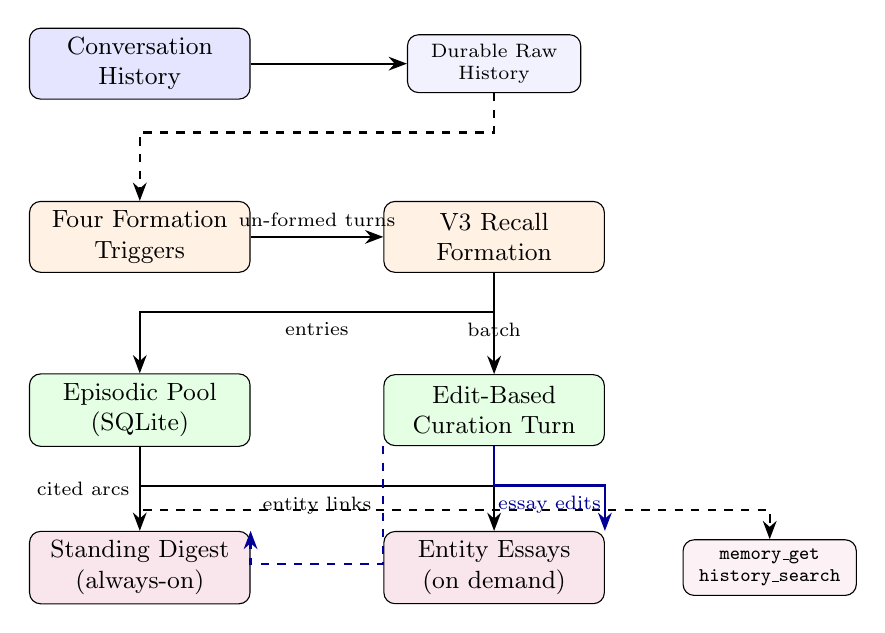
\begin{tikzpicture}[
    >=Stealth,
    box/.style={draw, rounded corners, minimum height=0.9cm,
                minimum width=2.8cm, align=center, font=\small},
    smallbox/.style={draw, rounded corners, minimum height=0.7cm,
                     minimum width=2.2cm, align=center,
                     font=\scriptsize},
    arrow/.style={->, thick},
    dasharrow/.style={->, thick, dashed},
    every node/.style={font=\small},
  ]

  % Row 0: Conversation
  \node[box, fill=blue!10] at (0, 0) (conv)
    {Conversation\\History};
  \node[smallbox, fill=blue!5] at (4.5, 0) (compact)
    {Durable Raw\\History};

  % Row 1: Formation pipeline
  \node[box, fill=orange!10] at (0, -2.2) (timer)
    {Four Formation\\Triggers};
  \node[box, fill=orange!10] at (4.5, -2.2) (segmenter)
    {V3 Recall\\Formation};

  % Row 2: Storage
  \node[box, fill=green!10] at (0, -4.4) (pool)
    {Episodic Pool\\(SQLite)};
  \node[box, fill=green!10] at (4.5, -4.4) (maps)
    {Edit-Based\\Curation Turn};

  % Row 3: Retrieval
  \node[box, fill=purple!10] at (0, -6.4) (toc)
    {Standing Digest\\(always-on)};
  \node[box, fill=purple!10] at (4.5, -6.4) (router)
    {Entity Essays\\(on demand)};
  \node[smallbox, fill=purple!5] at (8, -6.4) (tools)
    {\code{memory\_get}\\
     \code{history\_search}};

  % Arrows
  \draw[arrow] (conv) -- (compact);
  \draw[arrow, dashed] (compact.south) -- ++(0,-0.5) -| (timer.north);
  \draw[arrow] (timer) -- node[above, font=\scriptsize]
    {un-formed turns} (segmenter);
  \draw[arrow] (segmenter.south) -- ++(0,-0.5) -|
    node[pos=0.25, below, font=\scriptsize] {entries} (pool.north);
  \draw[arrow] (segmenter.south) -- ++(0,-0.5) -|
    node[pos=0.25, below, font=\scriptsize] {batch} (maps.north);
  \draw[arrow] (pool) -- node[left, font=\scriptsize]
    {cited arcs} (toc);
  \draw[arrow] (pool.south) -- ++(0,-0.5) -|
    node[pos=0.25, below, font=\scriptsize]
    {entity links} (router.north);
  \draw[dasharrow] (pool.south) -- ++(0,-0.8) -| (tools.north);
  \draw[arrow, blue!60!black] (maps.south) -- ++(0,-0.5) -|
    node[pos=0.25, below, font=\scriptsize, text=blue!60!black]
    {essay edits} (router.north east);
  \draw[dasharrow, blue!60!black] (maps.south west) -- ++(0,-1.5) -|
    (toc.north east);

\end{tikzpicture}
\caption{Current memory data flow. Startup, periodic, token-pressure, and
shutdown triggers feed V3 formation. Records commit to the episodic pool;
each successful batch queues a scoped curation turn that edits the standing
digest and active-entity essays. The raw log and episodic store remain
searchable beneath the curated text hierarchy.}
\label{fig:memory}
\end{figure}

\paragraph{Text hierarchy and governed procedure layer.}
\begin{description}[nosep, leftmargin=1.5em]
  \item[Conversation history] The durable raw message record and rolling
    context window. Context compaction may summarize the active window, but
    Formation~V3 consumes its own cursor over un-formed turns rather than
    treating window drops as a formation trigger.
  \item[Memory pool] Episodic memories stored in a SQLite database
    (\code{\textasciitilde/.mesh/memory/\{agent\}.db}). Each entry has
    three tiers of detail (Table~\ref{tab:memory-tiers}). The pool
    persists across sessions and grows over the agent's lifetime.
  \item[Standing digest] One per-agent Markdown briefing beneath
    \code{\textasciitilde/.mesh/digests/}. It is injected in place of the
    entry-level TOC and carries cross-project chronology, interpretation,
    durable decisions, live threads, and an agent narrative.
  \item[Entity essays] Cited narratives for active person, project, and
    event entities, stored in the per-agent SQLite database. They merge many
    linked episodes into a coherent, entity-specific account and are fetched
    through \code{essay\_list}/\code{essay\_get}.
  \item[Skill cards] Versioned YAML procedures under
    \code{\textasciitilde/.mesh/skills/}. Cards are selected separately from
    historical recall and are advisory until a human approves their lifecycle
    state.
\end{description}

\begin{table}[h]
\centering
\small
\begin{tabular}{@{}clL{7cm}@{}}
\toprule
\textbf{Tier} & \textbf{Name} & \textbf{Content} \\
\midrule
1 & Summary   & Short retrieval key (1 to 2 sentences). Always visible
                in the TOC. \\
2 & Reflection & Detailed analysis: what happened, why it matters,
                  lessons learned. Fetched via \code{memory\_get(id)}. \\
3 & Trace      & Full tool call trace from the original conversation.
                  Fetched via \code{memory\_get(id, full=true)}. \\
\bottomrule
\end{tabular}
\caption{Three-tier memory entry structure. Higher tiers are fetched on
demand to avoid context bloat.}
\label{tab:memory-tiers}
\end{table}

\section{Formation V3 Pipeline}

Memory formation converts un-formed conversation turns into structured
episodic entries. The V3 pipeline uses a dedicated LLM
(\code{memory\_llm\_backend}) that is decoupled from the agent's primary
worker backend. \code{mesh/memory/formation\_contract.py} is the single
prompt and parse authority shared by live formation and fold-compatibility
tooling.

\paragraph{Trigger and timing.}
Formation fires on four independent triggers (the defaults below are
configuration values, not provider requirements):
\begin{enumerate}[nosep]
  \item \textbf{Startup}: after memory initialization and embedding migration.
  \item \textbf{Timer}: every 1,800 seconds, deferring a tail younger than
        300 seconds so an exchange can finish.
  \item \textbf{Token pressure}: after roughly 30,000 newly appended,
        uncommitted tokens.
  \item \textbf{Shutdown}: one final blocking attempt with a 30-second cap.
\end{enumerate}
Under V3, \code{MemorySystemV2.on\_window\_drop()} explicitly does
\emph{not} form memories; it only updates rolling conversation-summary state.
This decoupling prevents context-compaction policy from controlling durable
memory formation.

\paragraph{Segmenter.}
The V3 segmenter (\code{mesh/memory/formation\_v3.py}) sends bounded,
overlapping windows of un-formed turns to the configured memory LLM. Defaults
are 60 turns per window with 20 turns of overlap and a 10-turn in-window defer
tail. The LLM returns a JSON array of records under the shared recall-oriented
contract. Each record contains:

\begin{itemize}[nosep]
  \item \code{topic\_label} --- concise label for the segment.
  \item \code{summary}, \code{reflection}, and \code{trace} --- the three
        episodic detail tiers.
  \item \code{retrieval\_key} --- compact search surface.
  \item \code{project} --- project assignment. The prompt encourages
        grounded labels but does not depend on a project map.
  \item \code{tags} --- categorization tags.
  \item \code{outcome} --- success, partial, or failure.
  \item \code{event\_date} --- the event's best date, distinct from the
        formation timestamp.
  \item \code{digest\_candidate} --- the second-bar signal described below.
  \item optional entity-resolution metadata when shadow or write mode is
        enabled.
\end{itemize}

\paragraph{Two bars.}
Formation is deliberately recall-oriented: it does not require or filter on a
1 to 10 ``worthiness score.'' Broadly useful events enter the episodic pool.
The higher precision bar is the boolean \code{digest\_candidate}; curation
uses it to decide which records may change always-on narrative context. This
separates ``worth remembering'' from ``worth occupying every future prompt.''

\paragraph{Cursor mechanics.}
A cursor index tracks which conversation turns have been processed.
Entry persistence and cursor advancement are atomic: if persistence
fails, the cursor stays put and the window is retried on the next
trigger. A cursor clamp prevents the cursor from advancing past the actual
history length after restarts. Empty-but-valid extraction may advance the
cursor, because it is a completed judgment rather than a parse failure.

\paragraph{Failure tolerance.}
A configurable strike counter tracks parse failures for one window. At the
default threshold of three, the system writes a visible placeholder entry
tagged \code{formation-fallback}, then advances. The failure therefore does
not wedge formation and is not silently erased as an ordinary ``skip.''

\paragraph{Cold-start handling.}
When project maps are disabled, formation continues normally: project
assignment is a field on each episodic record, not a dependency on map
creation. If the optional map subsystem is enabled, the retained compatibility
path may bootstrap and integrate maps after entry persistence.

\section{Edit-Based Self-Curation}
\label{sec:self-curation}

After a successful formation commit, \code{RouterV2} enqueues one internal
curation batch. A serialized drain loop processes those batches outside the
normal message lock, so an LLM maintenance call cannot starve interactive
traffic. The curation turn receives the new batch, the full active/pending
entity registry, bounded artifact measurements, and any durable additions
that a previous turn could not land.

\paragraph{Scoped update loop.}
The internal turn uses the existing router tool loop with a deliberately
narrow catalog. It may inspect memories, entities, essays, and the digest;
create/link/merge/retire entities; correct entity links; and apply exact
\code{digest\_edit} or \code{essay\_edit} replacements. Group mutations are
present only when the group feature is enabled. Every mutation runs under a
curation execution context (shadow or write mode), so normal interactive text
cannot silently acquire internal curation authority.

The turn has three responsibilities:
\begin{enumerate}[nosep]
  \item link the new records to existing entities or create grounded pending
        entity proposals;
  \item maintain essays for active entities using all linked evidence, not
        only the latest batch; and
  \item update the standing digest only with high-bar, agent-wide material,
        preserving exact memory citations.
\end{enumerate}

\paragraph{Digest constitution.}
\code{DIGEST\_CONSTITUTION} in \code{mesh/memory/curation.py} is the live
write authority. The digest must retain seven non-empty sections: Timeline,
Narrative, Projects, People, Standing decisions \& conventions, Open threads,
and Agent narrative. Timeline is chronological; Narrative is causal and
compressed by liveness; Standing decisions grow monotonically; Open threads
are rewritten as live state. Every \code{[m\_<12hex>]} citation must resolve
and support the particular claim it follows. The tracked companion source
\code{mesh/fold\_driver/prompts/standing\_digest/constitution.txt} supplies
the shared standing-digest rules used by formation/fold compatibility.

\paragraph{Essay constitution.}
Entity essays are the substantive narrative layer, not registry metadata.
Each entity type has a required structure; claims cite only records linked to
that entity. Publication is restricted to active entities and validates
citations, placeholders, evidence scope, concurrency version, and token
budget. Initial essay generation uses the same publish path and gets one
bounded repair attempt; ongoing changes use \code{essay\_edit}.

\paragraph{Nightly fold status.}
The old offline nightly fold is no longer the primary maintenance writer.
Digest and essay changes now land during these edit-based curation turns.
\code{mesh/fold\_driver/} and \code{mesh/memory/essay\_fold.py} remain as
tracked compatibility, bootstrap, and audit tooling, but a deployment should
not describe the retired chronological batch fold as the live digest path.

\section{Entity Registry and Cited Essays}

\code{mesh/memory/entities.py} owns a per-agent SQLite registry. Entity keys
are typed as person, project, event, or group and move through
pending/active/retired states. Aliases are Unicode-normalized; merges retain a
replacement key; memory links and correction events are transactional.
Activation is evidence-based: by default an entity must be observed across
three distinct formation windows, rather than repeated several times in one
window. The active-entity cap bounds registry growth.

The entity service is also the publication gate for essays. Before a write
commits it checks that the target is active, the evidence version is current,
every canonical memory ID resolves, every cited memory is linked to the
target, no loose or placeholder citation syntax remains, and the body fits
its ceiling. \code{mesh/memory/ids.py} normalizes accepted memory-ID surfaces
to the canonical 12-hex handle. These gates apply equally to generated and
hand-edited essays; no alternate write path bypasses them.

\section{Ceilings, Durable Carry-Forward, and Write Audit}

Curated artifacts have hard token ceilings. \code{ceiling\_rules.py}
implements a make-room-then-land contract: an over-ceiling write is refused,
never truncated, and the refusal carries an artifact-specific compaction
order plus an instruction to retry the same addition in the same turn. Digest
compaction merges old quiet Timeline ranges first, compresses Narrative by
liveness second, and tightens must-keep sections last without emptying them or
discarding the only surviving judgment. Essay compaction similarly preserves
cited conclusions over event-by-event detail.

If the model cannot land the addition in that turn,
\code{pending\_additions.py} writes the full, unclipped edit into the agent's
SQLite database at turn end. Up to eight oldest pending additions are offered
back on a later curation turn. A row resolves only when exact committed text
proves it landed, or when citation-preserving markers prove a compressed
replacement superseded it. The durable queue is bounded per artifact, rejects
lossy previews, and survives restarts with the rest of the memory store.

\code{write\_audit.py} records every curated-artifact write attempt in the
existing entity-event trail. Outcomes distinguish landed, refused, retried,
and queued attempts and include before/after hashes, token measurements, and
retry attribution. The audit can therefore compute retry success, terminal
drops, and carried-forward additions without changing the write decision.

\section{Retrieval}

Several retrieval paths expose different abstraction levels instead of
forcing every query through one index.

\paragraph{Always-on digest or TOC.}
When \code{standing\_digest\_enabled} is true, the validated digest is
injected in place of \code{<memory\_toc>}. If no standing digest is enabled,
the fallback TOC contains up to 30 representative episodic records. The
two-stage TOC algorithm remains implemented and is described in
Chapter~\ref{ch:maps-toc}.

\paragraph{On-Demand Tools.}
\begin{itemize}[nosep]
  \item \code{memory\_get(id)} --- fetches the full reflection (Tier 2)
        of a specific entry. The result persists in conversation history
        for the rest of the session.
  \item \code{memory\_search(query, project=...)} --- defaults to hybrid
        search: embedding similarity and SQLite FTS5/BM25 lexical rankings
        are merged by reciprocal-rank fusion. Explicit embedding-only and
        lexical-only modes remain available.
  \item \code{history\_search(query)} --- keyword search over durable raw
        conversation logs for details that were never formed or were omitted
        from a higher-level summary.
  \item \code{digest\_get}, \code{essay\_list}, and \code{essay\_get} ---
        retrieve curated context by agent or entity before opening granular
        episodes.
\end{itemize}

\paragraph{Router-Level Injection.}
Before dispatching work to a worker, the router runs
\code{\_select\_memory\_context()} to curate and inject relevant
memories into the worker's context. A small relevance-filtered set is
formatted as \code{<router\_injected\_context>} XML and prepended to the
worker prompt. Optional project-map context may be appended only when that
legacy subsystem is enabled.

\paragraph{Correction tools.}
The memory layer is mutable under explicit, audited operations. An
ID-stable \code{memory\_edit} re-embeds changed retrieval fields;
\code{memory\_delete} removes an episode and updates selection state;
\code{digest\_get}/\code{digest\_edit} maintain the standing briefing; and
essay edits run through entity citation and ceiling validators. Corrections
therefore change the agent-facing artifacts rather than merely appending a
contradictory raw-history message.

\section{Feature Flag Matrix}

Memory features are deployed incrementally per agent via configuration
flags in \code{mesh.yaml}. Formation V3 uses a dedicated LLM backend
(\code{memory\_llm\_backend}) decoupled from the agent's worker backend.
The current code independently gates V3 formation, standing-digest injection,
entity resolution (off/shadow/write), self-curation mode, essay generation,
groups, and legacy project maps. Configuration validation refuses self-
curation enrollment unless V3 formation and the standing digest are enabled
and project maps are disabled; this prevents two narrative writers from
competing for the same role.

\section{Standing Digest (Curation-Maintained)}
\label{sec:standing-digest}

The standing digest extends the memory system with a dense, continuously
updated summary document per agent. Where the episodic memory pool
stores individual entries with three-tier retrieval, the standing digest
is a single coherent narrative (a ``standing briefing'') that captures
the agent's full operational history, key decisions, project context, and
relationship knowledge in one document.

\paragraph{Architecture.}
The live writer is the curation turn in
\code{mesh/memory/curation.py}. It proposes exact edits after successful
formation batches; \code{AgentNode} validates section structure, citations,
the measured token ceiling, and write authority before an atomic update.
Over-ceiling refusals must compact and retry or enter the durable
pending-additions ledger. The old cursor-driven offline fold remains
available for compatibility and bootstrap work, not as the normal nightly
maintenance path.

\paragraph{Configuration.}
The live surface is centered on:
\begin{itemize}[nosep]
  \item \code{standing\_digest\_enabled} (bool) --- when true, the
        published digest replaces the \code{<memory\_toc>} block in the
        agent's system prompt.
  \item \code{standing\_digest\_path} (str) --- path to the published
        digest file (Markdown).
  \item \code{entity\_self\_curation\_mode} --- off, shadow, or write mode
        for internal mutations.
  \item curation tool/iteration, essay, group, and failure-alert limits ---
        bounded independently from normal message turns.
\end{itemize}

\paragraph{Quality gates.}
Each write checks citation provenance (every \code{[m\_...]} handle resolves),
the seven required non-empty sections, exact replacement semantics, and the
measured ceiling. Curation instructions add claim-to-citation correspondence,
chronological Timeline ordering, recent-coverage review, and graduation rules
that forbid deletion of the only surviving judgment. Write auditing records
both successful and refused attempts.

\paragraph{Relationship to episodic memory.}
The standing digest and the episodic memory pool are complementary, not
competing. The pool stores granular entries for on-demand retrieval; the
digest provides always-on holistic context. When \code{standing\_digest\_enabled}
is true, the digest replaces the TOC injection (which would otherwise
list individual entry summaries), while the pool's search and retrieval
tools remain available.

\section{Governed Procedural Memory}

\code{mesh/procedural\_memory.py} stores procedures as versioned YAML
\emph{skill cards}, separate from episodic facts and entity narratives. A card
records triggers, typed preconditions, authority, source files and SHA-256
fingerprints, required invariants, verification, rollback, evidence, and an
append-only outcome history.

The lifecycle is \code{proposed} $\rightarrow$ \code{active}
$\rightarrow$ \code{retired}, but the runtime deliberately exposes no
activation API. \code{skill\_draft} can package a completed worker trace and
source evidence into a proposal; a human must review the file and supply
approval metadata before it becomes active. Source-fingerprint drift
suppresses stale cards.

Selection is deterministic and advisory. Required typed preconditions are
checked for contradictions first; contradicted cards are excluded. Eligible
cards are then ranked by BM25-like text relevance with stricter treatment of
unknown required facts, and at most three are injected. The rendered block
explicitly grants no additional authority and never auto-executes a procedure.
Outcome receipts support later meta-review without converting observed success
into automatic policy.

\section{Key Files}

\begin{table}[h]
\centering
\small
\begin{tabular}{@{}lL{7cm}@{}}
\toprule
\textbf{File} & \textbf{Purpose} \\
\midrule
\code{mesh/memory/system\_v2.py}
  & Core formation orchestration, episodic retrieval, TOC/FL selection,
    correction operations, and optional map compatibility. \\
\code{mesh/memory/formation\_v3.py}
  & V3 segmenter: JSON-structured LLM segmentation with validation,
    clamping, and retry logic. \\
\code{mesh/memory/formation\_contract.py}
  & Shared low-bar prompt, canonical record fields, entity envelope, and
    response parser. \\
\code{mesh/memory/store.py}
  & SQLite persistence: \code{MemoryEntry} dataclass, CRUD operations,
    FTS5 index, entities, essays, pending additions, wakes, and maps. \\
\code{mesh/memory/entities.py}
  & Per-agent entity registry, link correction, merge/retirement,
    preflight validation, and cited-essay publication gates. \\
\code{mesh/memory/entity\_essays.py}, \code{essay\_fold.py}
  & Canonical essay generation/publication plus retained fold compatibility. \\
\code{mesh/memory/curation.py}
  & Scoped edit-based curation batches, digest/essay constitutions, shadow and
    write execution contexts. \\
\code{mesh/memory/ceiling\_rules.py}
  & Artifact-specific make-room-then-retry refusals. \\
\code{mesh/memory/pending\_additions.py}
  & Durable queue and evidence-based resolution for un-landed additions. \\
\code{mesh/memory/write\_audit.py}
  & Per-attempt outcome, hash, token, retry, and drop-rate audit records. \\
\code{mesh/memory/ids.py}
  & Canonical 12-hex memory-handle normalization. \\
\code{mesh/memory/selection.py}
  & FLMI active set selection using embedding vectors. \\
\code{mesh/memory/embeddings.py}
  & Embedding client for memory entry vectorization. \\
\code{mesh/procedural\_memory.py}
  & Governed YAML skill-card schema, human lifecycle, selection, receipts,
    source-drift suppression, and proposal drafting. \\
\code{mesh/paths.py}
  & Central path resolution for memory, digests, maps, skills, and isolated
    agent state. \\
\code{mesh/prompts/memory.md}
  & Shared prompt instructions for memory, digest, essay, and history tools. \\
\bottomrule
\end{tabular}
\caption{Memory system source files.}
\label{tab:memory-files}
\end{table}


%----------------------------------------------------------------------
\chapter{TOC Selection and Optional Project Maps}
\label{ch:maps-toc}
%----------------------------------------------------------------------

\section{Compatibility Status of Project Maps}

Project maps remain implemented, but they are an optional legacy narrative
subsystem rather than a tier in the v2 self-curation hierarchy. When enabled,
maps are Markdown files beneath
\code{\textasciitilde/.mesh/memory/maps/} with summary/embedding metadata in
SQLite. Formation can asynchronously bootstrap an unknown project and
integrate a multi-project entry batch through full-section replacement or
section append operations. Integration failure is non-blocking with respect
to episodic persistence and cursor advancement.

The retained canonical map schema is Summary, Goals, Architecture, Key Files,
Key Decisions, Current State, Open Issues, and Glossary. Self-curation
enrollment validation requires \code{project\_maps\_enabled=false}, because
the curation-maintained digest and project/entity essays now own the durable
narrative role. Deployments that keep maps enabled may still use the routing
and selection mechanics below.

\section{Relevance-Based Map Injection}
\label{sec:map-injection}

When \code{project\_maps\_injection\_enabled} is true, project maps are
injected into router and worker prompts based on relevance to the current
conversation, replacing the earlier approach of injecting only the
statically tracked \code{\_active\_project} map.

\paragraph{Algorithm.}
\begin{enumerate}[nosep]
  \item Concatenate the text of the last $N$ conversation turns
        ($N{=}5$ by default, hardcoded in the router's
        \code{\_get\_last\_n\_turns\_text()} helper).
  \item Embed the concatenated text using the memory embedding client
        (\code{text-embedding-3-small}).
  \item Compute cosine similarity between the context embedding and each
        project map's summary embedding (stored in the
        \code{project\_maps} table).
  \item Return the top-$k$ maps ($k{=}2$) with similarity above a
        minimum threshold (0.2).
\end{enumerate}

\paragraph{Injection points.}
\begin{itemize}[nosep]
  \item \textbf{Router prompt}: \code{\_build\_system\_prompt()} and
        \code{\_build\_router\_prompt()} call
        \code{render\_relevant\_maps\_block()} (which wraps
        \code{select\_relevant\_maps()}), injecting up to~2 maps as
        \code{<project\_map project="..." relevance="...">} blocks.
  \item \textbf{Worker prompt}: \code{\_select\_memory\_context()}
        appends relevant maps to the
        \code{<router\_injected\_context>} block alongside memory
        entries. Workers previously received no project maps.
  \item \textbf{Fallback}: if no map embeddings are available (embedder
        down, or maps lack summaries), falls back to
        \code{render\_maps\_block()} (active project only).
\end{itemize}
Every path first checks the map-injection feature gate; disabled means an
empty block, not an active-project fallback.

\paragraph{Summary embeddings.}
Each project map maintains a 1 to 2 sentence summary in the
\code{project\_maps.summary} column, extracted deterministically from
the map's \code{\#\# Summary} section after every content change.
The summary is embedded via \code{text-embedding-3-small} and stored in
the \code{embedding} BLOB column.
Summaries are better embedding targets than full map content: they
capture the project's domain and focus in a dense, semantically rich
form, whereas full maps contain structural/list content that dilutes
embedding quality.

\paragraph{Design rationale.}
The static \code{\_active\_project} approach had two limitations:
(1) only one map was ever injected, even when conversations spanned
multiple projects, and (2) workers received no project context at all.
Relevance-based selection aligns map injection with the same principle
used for memory entry retrieval.

\section{TOC Selection and Weighting (FLMI)}

When the standing digest is disabled, up to 30 entries shown in the prompt
TOC are selected from the full pool using a two-stage pipeline that balances
breadth with diversity. With a standing digest, this remains a fallback and
diagnostic mechanism rather than the normal always-on prompt block.

\paragraph{Stage 1: Cosine relevance.}
The top~100 entries by cosine similarity to the last $N$ conversation
turns are selected as candidates. This ensures the TOC is grounded in
the current conversational context.

\paragraph{Stage 2: Facility Location diversity.}
From the top-100 candidates, the \code{lazy\_greedy\_fl()} function
(in \code{mesh/memory/selection.py}) selects 30 entries using a
submodular Facility Location objective. This maximizes embedding
diversity, ensuring broad coverage of the agent's topic history rather
than clustering around a single recent topic.

\paragraph{Representative-set distinction.}
The older persistent active-set selector can starve a redundant new entry of
facility-location gain. The query-conditioned TOC path does not treat that
active set as a pool ceiling: it first restricts the full candidate pool by
the current query, then runs \code{lazy\_greedy\_fl()} inside that top-100
set. This preserves the useful diversity objective without describing the
legacy active set as the whole memory hierarchy.

\paragraph{Summary maintenance.}
When the optional subsystem is enabled, each project map has a short summary
(1 to 2 sentences) stored alongside
an embedding vector in the \code{project\_maps} table. Summaries are
extracted deterministically after every map content change (via
integration, tool edits, or manual curation) by parsing the canonical
\code{\#\# Summary} section from the map content (no LLM call needed).
If no \code{\#\# Summary} section exists, the first non-heading
paragraph (up to 500 characters) is used as a fallback. The embedding
is recomputed from the updated summary and cached in memory. The update
runs as a fire-and-forget \code{asyncio.create\_task}.


%======================================================================
%======================================================================
\part{Infrastructure and Operations}
\label{part:infrastructure}
%======================================================================
%======================================================================

%----------------------------------------------------------------------
\chapter{Multi-Host Deployment}
\label{ch:deployment}
%----------------------------------------------------------------------

The mesh system supports multi-host deployments where a central router
coordinates agents running on separate machines. This chapter documents
the deployment topology patterns, service management, and cross-host
coordination mechanisms. See also \code{docs/two-host-demo.md} for a
concrete walkthrough.

\paragraph{Typical topology.}
A production deployment assigns distinct roles to hosts:
\begin{description}[nosep, leftmargin=1.5em]
  \item[Primary host] Runs the router (optionally systemd-managed),
    multiple agents, an nginx reverse proxy with TLS termination, and the
    web client.
  \item[Secondary host(s)] Run additional agents. Connected to the
    primary via WebSocket (optionally through an nginx proxy for TLS).
  \item[Backup target] (optional) Receives daily incremental rsync
    snapshots from the primary host.
\end{description}

\paragraph{Service management.}
The router and critical agents can be managed via systemd units with
automatic restart on failure. Other agents are managed via
\code{agent-ctl.sh}, a shell script providing start/stop/status
operations with backend selection.

\paragraph{Cross-host sync.}
Syncthing or similar tools can synchronize \code{\textasciitilde/.mesh}
and shared directories across hosts. This ensures memory databases
and configuration changes propagate automatically. The application code
can be synchronized via git.

\paragraph{Backup.}
A daily incremental rsync job can copy the mesh state to a backup target
with configurable retention.


%----------------------------------------------------------------------
\chapter{Security Hardening}
\label{ch:security}
%----------------------------------------------------------------------

Several hardening measures protect subprocess spawning, credential
handling, and inter-process communication.

\section{Subprocess Environment Allowlist}

All LLM subprocess methods (\code{\_run\_cc\_subprocess},
\code{\_complete\_codex}, \code{\_complete\_mesh\_harness},
\code{cc\_session.py}, \code{router\_cc.py}, \code{eval/evaluator.py})
filter \code{os.environ} through \code{\_build\_subprocess\_env()}, a
module-level helper in \code{mesh/llm.py}. The allowlist is a
\code{frozenset} of~30 approved environment variables plus prefix
matching for \code{CLAUDE\_*} and \code{ANTHROPIC\_*}.

\begin{table}[h]
\centering
\small
\begin{tabular}{@{}lL{8cm}@{}}
\toprule
\textbf{Category} & \textbf{Allowed Variables} \\
\midrule
System     & \code{PATH}, \code{HOME}, \code{USER}, \code{SHELL},
             \code{LANG}, \code{LC\_*}, \code{TERM}, \code{TMPDIR},
             \code{XDG\_*}, \code{SSH\_AUTH\_SOCK} \\
API keys   & \code{OPENAI\_API\_KEY}, \code{ANTHROPIC\_API\_KEY},
             \code{DEEPSEEK\_API\_KEY}, \code{EXA\_API\_KEY},
             \code{ZAI\_API\_KEY}, \code{OPENROUTER\_API\_KEY},
             \code{SYNTHETIC\_API\_KEY}, \code{GOOGLE\_API\_KEY} \\
Mesh       & \code{MESH\_AUTH\_TOKEN}, \code{MESH\_NODE\_ID},
             \code{MESH\_ATTACHMENT\_SECRET} \\
Python     & \code{VIRTUAL\_ENV}, \code{PYTHONDONTWRITEBYTECODE},
             \code{PYTHONHASHSEED} \\
\bottomrule
\end{tabular}
\caption{Subprocess environment allowlist categories. Variables not in this
list (e.g., \code{LD\_PRELOAD}, \code{LD\_LIBRARY\_PATH},
\code{PYTHONPATH}) are blocked.}
\label{tab:env-allowlist}
\end{table}

\noindent
Operator-controlled overrides (\code{cc\_env}, \code{env\_override} in
\code{LLMConfig}) are applied \emph{after} filtering and may inject
arbitrary variables by design (e.g., account-specific \code{HOME},
custom API keys).

\section{API Key Masking in Logs}

The \code{\_mask\_cmd()} helper in \code{mesh/llm.py} masks sensitive
values in subprocess command logs. It handles both two-token
(\code{-{}-api-key VALUE}) and single-token (\code{-{}-api-key=VALUE})
forms, replacing values with \code{***} plus the last 4 characters.
Only log output is affected; the actual subprocess command is unchanged.

\section{Socket Path Hardening}

Agent tool sockets moved from the world-readable \code{/tmp/} directory
to \code{\textasciitilde/.mesh/sockets/} with directory mode~0700
(owner-only). Socket names are deterministic
(\code{\{sanitized\_node\_id\}.sock}) within the restricted directory---
no random suffix needed since only the owning user can list or connect.

\section{Node ID Propagation}

\code{MESH\_NODE\_ID} is set via two independent paths:
\begin{enumerate}[nosep]
  \item \textbf{Process-level}: \code{os.environ["MESH\_NODE\_ID"]}
        set in \code{AgentNode.\_\_init\_\_} for tool subprocess
        inheritance.
  \item \textbf{Per-LLMClient}: \code{LLMConfig.node\_id} injected
        explicitly into each LLM subprocess environment. Ensures
        correctness if multiple \code{LLMClient} instances exist in one
        process.
\end{enumerate}

\section{Agent Node Refactoring}

The 842-line \code{\_process\_with\_llm} method was decomposed into a
280-line orchestrator plus six focused helpers:

\begin{itemize}[nosep]
  \item \code{\_setup\_controller\_for\_message} --- controller
        initialization and streaming observer.
  \item \code{\_build\_system\_prompt\_for\_llm} --- memory, preferences,
        personality, trace prompt assembly.
  \item \code{\_build\_worker\_instructions} --- worker instructions and
        briefing mode setup.
  \item \code{\_handle\_controller\_llm\_response} --- controller
        decision routing.
  \item \code{\_dispatch\_special\_tool\_calls} --- 10 special tool types
        (send\_message, schedule\_wake, etc.).
  \item \code{\_process\_tool\_calls\_in\_loop} --- full tool iteration
        processing with retry and error handling.
\end{itemize}

\section{Confirmation Gate Bypass}

Two mechanisms allow tool calls to skip interactive confirmation:

\begin{enumerate}[nosep]
  \item \textbf{Socket handler \code{skip\_confirmation=True}}
    (\code{agent\_node.py}): When a worker subprocess calls a
    confirmation-required tool (e.g., \code{gmail\_send\_message}) via
    the agent socket, the socket handler executes it with
    \code{skip\_confirmation=True}. The rationale is that the user already
    authorized the work by dispatching the worker; re-prompting for
    confirmation on each sub-action would make the worker unusable.

  \item \textbf{\code{auto\_confirm\_tools} config}: Per-agent YAML
    configuration that lists tool names which should always skip
    confirmation for that agent. Used for Alice's Gmail write tools in
    production.
\end{enumerate}

\noindent Both mechanisms are intentional design decisions, not security
bypasses. The trust boundary is at worker dispatch time, not at
individual tool invocation time within an authorized worker session.


\section{IDLE$\to$BUSY Race Fix}

In \code{router\_v2.py}, the worker task is now created
\emph{before} \code{self.\_state} is set to \code{BUSY}. Since asyncio
is single-threaded, the task does not execute until the next yield, but
the invariant \code{\_state == BUSY $\implies$ \_worker\_task is not
None} now holds at every point.


%----------------------------------------------------------------------
\chapter{Benchmark Infrastructure}
\label{ch:benchmarks}
%----------------------------------------------------------------------

The mesh includes a benchmark harness for systematic evaluation of
backend configurations against a curated test suite. This chapter
documents the infrastructure; results are presented in
Chapter~\ref{ch:results}.

\paragraph{Runner.}
\code{benchmark/run\_sanity\_mesh\_harness.py} is the main entry point.
It accepts a \code{-{}-mesh-backend} argument specifying which
\code{mesh.yaml} backend to evaluate, plus optional flags for thinking
budget, assessor effort, and codex assessor configuration. The runner
iterates over a suite of test instances, launching the harness
subprocess for each, collecting patches, and running evaluation
(typically \code{pytest} inside a Docker container matching the target
repository).

\paragraph{Backend resolution.}
\code{benchmark/\_mesh\_backend.py} defines \code{ResolvedBackend}, a
dataclass that resolves a backend name from \code{mesh.yaml} into a
complete configuration including model, API endpoint, controller mode,
soft limit, thinking budget, and assessor configuration.

\paragraph{Test suites.}
The primary suite is \code{benchmark/delta\_suite.json}, a 15-instance
collection covering 10 hello-world instances (drawn from real mesh
system bugs) and 5 SWE-bench instances (astropy, django, ansible, etc.).
Additional suites exist for research benchmarks and full SWE-bench
evaluation.

\paragraph{Evaluation.}
Each instance includes a test specification. After the harness produces
a patch, the runner applies it to a clean checkout inside a Docker
container and runs the test suite. Results are recorded as pass/fail
counts per instance, along with token usage, wall time, and iteration
counts.


%======================================================================
%======================================================================
\part{Evaluation}
\label{part:evaluation}
%======================================================================
%======================================================================

%----------------------------------------------------------------------
\chapter{Benchmark Results and Ablations}
\label{ch:results}
%----------------------------------------------------------------------

This chapter will present empirical results from benchmark evaluations
of different backend configurations, including ablations over thinking
budgets, assessor effort levels, and controller modes. Key comparisons
include:

\begin{itemize}[nosep]
  \item \textbf{Standard vs.\ P\&E mode} on the 15-instance delta
        suite, with per-instance breakdowns showing where the assessor
        adds value and where it regresses.
  \item \textbf{Thinking budget ablation} (Qwen3.6-27B with and without
        \code{thinking\_budget: 16384}): standard mode improved from
        9/15 (60\%) to 11/15 (73\%) with thinking enabled, while P\&E
        held at 12/15 (80\%) with different failure composition.
  \item \textbf{Heterogeneous backend combinations}: local Qwen executor
        with DS-pro API assessor, GLM-5.1 executor with DS-pro assessor,
        and monolithic API-only configurations.
  \item \textbf{Wall time and cost analysis}: standard + thinking at
        82 min vs.\ P\&E at 220 min for similar accuracy on a free local
        model.
\end{itemize}


%----------------------------------------------------------------------
\chapter{Lessons Learned}
\label{ch:lessons}
%----------------------------------------------------------------------

This chapter documents operational lessons from running the mesh
system in production across multiple agents for 5+ months.

\begin{itemize}[nosep]
  \item \textbf{Memory retrieval adoption}: Despite a well-populated
        memory pool (450+ entries across agents), active retrieval
        (\code{memory\_get}, \code{memory\_search}) remained at zero
        for 24+ hours post-deployment. Root cause: CC-backend agents
        lack native tool access to memory tools; the CLI bridge is
        high-friction. Passive channels (TOC injection, router injection)
        carried the load.
  \item \textbf{Project mis-tagging}: Formation V3's conservative
        prompt (``Do NOT invent new identifiers'') caused entries to
        collapse into a single project. Fixed by encouraging
        organic project creation and removing the
        \code{\_active\_project} null fallback.
  \item \textbf{P\&E overhead}: The assessor consumes up to 65\% of
        total tokens. For simple tasks, standard mode with thinking
        enabled matches P\&E accuracy at 2.7x lower wall time.
  \item \textbf{Agent coordination}: Ack-to-ack loops between agents
        in channels required explicit suppression rules. Agents
        defaulted to acknowledging each other's messages, creating
        unbounded ping-pong chains.
  \item \textbf{Standing digest vs.\ TOC}: The episodic memory TOC
        (always-on entry summaries) scales poorly past several hundred
        entries. The curation-maintained standing digest
        (Section~\ref{sec:standing-digest}) resolved this by replacing
        the entry-level TOC with a single coherent narrative, trading
        per-entry granularity for holistic context while retaining hybrid
        search and exact memory handles underneath.
  \item \textbf{Harness-backend router dispatch}: When the router itself
        runs on a harness backend (Claude Code, Codex), the native
        tool-call dispatch path is unavailable. The unified dispatch
        contract (\code{<dispatch\_worker>} XML blocks, stripped router
        tools, single outer iteration) emerged from repeated failures
        where harness-backend routers attempted to call tools they could
        not execute.
\end{itemize}


\end{document}
